\documentclass[11pt,oneside,openany,a4paper,english, report, goldenblock
]{usthesis}
\usepackage{enumerate}
\usepackage[hmargin={25mm,20mm},vmargin={20mm,20mm}]{geometry}
\usepackage{helvet}
\usepackage[nobottomtitles*]{titlesec}
\usepackage{lipsum}
\usepackage{fancyhdr}
\usepackage{varioref}
\usepackage[english]{babel}
\usepackage[latin1]{inputenc}%.. Recognizes ê, ë, etc
\usepackage{amsmath} %.. Advanced maths (before fonts)
\usepackage{mathtools}
\usepackage[T1]{fontenc} %.. Type 1 fonts for proper hyphenation
\usepackage{textcomp} %.. Additional text characters
\usepackage{fourier} %.. Utopia (if you want a different font)
\usepackage{bm} 
\usepackage{graphicx}
\usepackage{color}
\usepackage{usbib}
\usepackage{natbib}
\usepackage{floatrow}%
\usepackage[onehalfspacing]{setspace}
\usepackage{subfig}
\usepackage{hyperref}
\usepackage[labelfont=bf]{caption}
\usepackage[shortlabels]{enumitem}
\usepackage[acronym,toc]{glossaries}
\usepackage{xspace}
\usepackage{listings}
\usepackage{color}
\usepackage[section]{placeins}

\definecolor{codegreen}{rgb}{0,0.6,0}
\definecolor{codegray}{rgb}{0.5,0.5,0.5}
\definecolor{codepurple}{rgb}{0.58,0,0.82}
\definecolor{backcolour}{rgb}{0.95,0.95,0.92}

\lstdefinestyle{mystyle}{
	%backgroundcolor=\color{backcolour},   
	commentstyle=\color{codegreen},
	keywordstyle=\color{magenta},
	numberstyle=\tiny\color{codegray},
	stringstyle=\color{codepurple},
	basicstyle=\footnotesize,
	breakatwhitespace=false,         
	breaklines=true,                 
	captionpos=b,                    
	keepspaces=true,                 
	numbers=left,                    
	numbersep=5pt,                  
	showspaces=false,                
	showstringspaces=false,
	showtabs=false,                  
	tabsize=2
}
\lstset{style=mystyle}

\titleformat
{\chapter} % command
[display] % shape
{\bfseries\Large\centering} % format
{CHAPTER \ \thechapter} % label
{-2ex} % sep
{
	\vspace{1.5ex}
	\centering
	\uppercase
} % before-code
[
\vspace{-2ex}%
] % after-code

\titlespacing*{\chapter}{0pt}{-15pt}{40pt}

\newcommand\applyappendixstyling{%
	\titleformat
	{\chapter} % command
	[display] % shape
	{\bfseries\Large\centering} % format
	{APPENDIX \ \thechapter} % label
	{-2ex} % sep
	{
		\vspace{1.5ex}
		\centering
		\uppercase
	} % before-code
	[
	\vspace{-2ex}%
	] % after-code
	
	\titlespacing*{\chapter}{0pt}{-15pt}{40pt}
}


\titleformat{\section}
{\normalfont\bfseries\uppercase}
{\thesection.}{0.5em}{}

\fancyhf{}
\fancyhead[C]{\thepage}
\pagestyle{fancy}
\renewcommand\headrulewidth{0pt}
\setlength{\headheight}{20pt}

\fancypagestyle{plain}{%
	\fancyhf{}
	\fancyhead[C]{\thepage}
	\pagestyle{fancy}
	\renewcommand\headrulewidth{0pt}
	\setlength{\headheight}{20pt}
}

\usepackage[toc,page]{appendix}

\renewcommand{\familydefault}{\sfdefault}
\setlength{\parskip}{0.5em}
\setlength{\parindent}{0pt}



% Acronyms:
\newacronym{ann}{ANN}{artificial neural network}
\newacronym{cnn}{CNN}{convolutional neural network}
\newacronym{rnn}{RNN}{recurrent neural network}
\newacronym{sde}{SDE}{stochastic differential equation}
\newacronym{mlestimation}{MLE}{maximum likelihood estimation}
\newacronym{mle}{MLE}{maximum likelihood estimate}
\newacronym{mme}{MME}{generalised method of moments estimation}
\newacronym{elu}{ELU}{exponential linear unit}
\newacronym{relu}{ReLU}{rectified linear unit}
\newacronym{em}{EM}{expectation maximisation}
\newacronym{gbm}{GBM}{geometric Brownian motion}
\newacronym{gpu}{GPU}{graphics processing unit}
\newacronym{aws}{AWS}{Amazon Web Services}
\newacronym{ec2}{EC2}{Elastic Compute Cloud}

\makeglossaries

%opening
\title{A Universal Calibration Scheme for Stochastic Processes using Artificial Neural Networks}
\author{R.W. Mostert}{Rayno Willem Mostert}
\faculty{Faculty of Economic and Management Sciences}
\degree{BCom Hons (Actuarial Science)}

\begin{document}
	\pagenumbering{roman}
	\supervisor{Mr. Stuart Reid \and Mr. Stephen Burgess}
	\ReportDescript{Thesis presented in partial fulfilment of the requirements for the degree of BCommHons(Actuarial Science) in the Faculty of Economic and Management Sciences at Stellenbosch University}
	
	\TitlePage%
	
	\DeclarationDate{July 2017}
	\DeclarationPage
	

\
\begin{abstract}
	Stochastic processes are powerful tools which can be applied to almost any time series-related problem. They offer clear representations of real-world processes in ways in which deterministic formulae cannot. Yet, the underlying mathematics complicate their application. One aspect of particular concern is the calibration of these processes to real-world data sets. Common calibration methods, including \acrfull{mlestimation} and the \acrfull{mme}, can break down under more complex stochastic processes. \acrshort{mlestimation}, for example, requires the derivation of the likelihood function, which often requires a deep understanding of stochastic calculus.
	
	This dissertation proposes the use of \acrlong{ann}s (\acrshort{ann}s) as an alternative calibration method. The results obtained in the simulation study demonstrate the ability of \acrshort{ann}s to act as a calibration scheme for a complex stochastic process - the Merton Jump-Diffusion process. The ultimate hope is that \acrshort{ann}s might offer a universal calibration scheme for any stochastic process.
	
	The project starts by introducing stochastic processes and \acrshort{ann}s, followed by an analysis of the simulation study performed on the Merton Jump-Diffusion process. The performance of the \acrshort{ann} models are then compared to that of traditional calibration procedures.
\end{abstract}

\tableofcontents

\listoffigures

\listoftables

\printglossary[type=\acronymtype, title=List of abbreviations and/or acronyms, toctitle=List of abbreviations]
	
\chapter{Introduction} 
\label{chapter:introduction}
\pagenumbering{arabic}

\section{Introduction}

\begin{quote}
	Stochastic processes are becoming more important to actuaries: they underlie much of modern finance, mortality analysis and general insurance. They are immensely useful because they form the common language of workers in many areas that overlap in actuarial science.  It is precisely because most financial and insurance risks involve events unfolding as time passes that models based on processes turn out to be most natural.
	\\ --- Submission to the Faculty of Actuaries students' society in 1998 (\citefullauthor{cairns1998stochastic}; \citeyear{cairns1998stochastic})
\end{quote}

Stochastic processes are simply a collection of random variables, usually indexed by time \citep{Barone-Adesi}. They are typically used during the modelling process, in order to describe the evolution of an underlying real-world process. To allow for it to be used within the modelling context, a stochastic process is often expressed by its \acrfull{sde}. 
Using the \acrshort{sde}, the simulated stochastic process can then be adjusted to best represent the real-world process at hand - whether that be the evolution of the price of a certain stock, the claims on an insurance policy or the mortality rate of a group of policyholders. 
\citefullauthor{Oreskes} (\citeyear{Oreskes}) refer to this procedure of "[manipulating] the independent variables to obtain a match between the observed and simulated distribution or distributions of a dependent variable or variables", as model calibration.


Effectively modelling a real-world process involves two major challenges. Firstly, choosing an appropriate stochastic process with properties that mimic those of the real-world process; and, secondly, finding the most suitable parameters for the relevant \acrshort{sde}. In practice, however, the selection of an appropriate stochastic process is often influenced by the ease with which its parameters can be calibrated. Thus complex stochastic processes, with more complex \acrshort{sde}s, are often substituted for simpler, easily calibrated models. This can lead to the use of models that are subject to simplifying assumptions or possess properties that may not be the best possible representation of reality.


The difficulty associated with model calibration depends on the method of calibration applied. \citet{Mongwe} and \citet{Honore} describe how common calibration methods, including \acrfull{mlestimation} and the \acrfull{mme}, can break down under more complex \acrshort{sde}s. \acrshort{mlestimation}, for example, requires the derivation of the likelihood function, which is often difficult in the case of complex \acrshort{sde}s as they can yield unbounded likelihood functions.


Another calibration method that has seen a renaissance in the last decade is that of backpropagation, which has proven to be a powerful gradient descent-based algorithm for calibrating \acrlong{ann}s (\acrshort{ann}s). 
This paper will explore the ways in which these statistical learning techniques - namely \acrshort{ann}s, calibrated by backpropagation - could, in turn, be applied to the calibration of stochastic processes.



\section{Problem Statement}
Every stochastic process contains a set of parameters, $ Z $, which controls the dynamics of the paths produced by the model. The calibration problem can be framed as a mapping from the observed data, $ D $, or some transformation thereof, to these parameter values, $ Z $. Let $C$ denote the calibration method, then $C$ is necessarily of the form,

\begin{equation}
C:f \left( D \right) \rightarrow Z
\end{equation}

An \acrshort{ann} is a collection of interconnected processing units \citep{Teugels}, which realises a nonlinear mapping from inputs, $ R^X $ to outputs, $ R^Y $.

\begin{equation}
\acrshort{ann}: R^X \rightarrow R^Y
\end{equation}

This mapping is achieved by chaining a sequence of nonlinear multiple regression functions, f, (called activation functions) together in layers (see 1.5.1 below).


From equations (1.1) and (1.2), we can see that an \acrshort{ann} has the ability to estimate the calibration function, $ C $. 
This assertion is justified by the Universal Approximation Theorem, which states that "standard multilayer feedforward networks are capable of approximating any measurable function to any desired degree of accuracy" (\citefullauthor{Hornik},\citeyear{Hornik}).


The question, however, remains as to what such a network might look like and how it would compare to traditional calibration techniques.

\section{Research Objectives}
This paper has the primary objective of researching and testing the viability of \acrshort{ann}s as a universal method of parameter estimation for any stochastic process. As to be seen in the literature review, \acrshort{ann}s have been used extensively in the world of financial modelling, and to some extent in the calibration of simple stochastic processes.


Conceivably, \acrshort{ann}s have the potential to act as a universal calibration method for any stochastic process. This paper aims to investigate whether and how that might function in practice.


This study will consist of two phases. In the first, an \acrshort{ann} will be implemented for a sufficiently complex \acrshort{sde}, for which a likelihood function does exist (for comparative purposes). In the second phase, the accuracy of the network's approximation of the calibration function will be measured and compared against that of other calibration techniques.

\section{Importance of the Study}

An \acrshort{ann}-based approach to parameter estimation could likely provide numerous benefits above the popular \acrshort{mlestimation} and \acrshort{mme} approaches.
The technique could potentially provide a universal solution to approximate the calibration function, $C$, for any arbitrarily complex \acrshort{sde}.
It does not require the derivation of the likelihood function, which can be difficult.
The model drops some of the strong assumptions made by \acrshort{mlestimation} and \acrshort{mme}. 


Another possible advantage could lie in the scheme's ability to combine the predictive power of \acrshort{ann}s with the descriptive properties of certain stochastic processes. \citet{Olden} explain that "although in many studies \acrshort{ann}s have been shown to exhibit superior predictive power compared to traditional approaches, they have also been labelled a 'black box' because they provide little explanatory insight into the relative influence of the independent variables in the prediction process". The approach, whereby the \acrshort{ann} is used only to calibrate a more expressive and widely understood model - a stochastic process - might help to remedy this.


\citet{Mongwe} presents the example of the Merton Jump-Diffusion process with \acrshort{sde},

\begin{equation}
	d \ln{S_t}= \left( \mu - \frac{1}{2} \sigma^2 \right )dt+\sigma dB +d \left( \sum_{i=1}^{N_t} Y_i \right )
\end{equation}

where $ \mu $  is referred to as the drift coefficient and $ \sigma $ as the diffusion coefficient. $ B_{t}, t\geq 0$ is a standard \acrfull{gbm} process. $Y_i$ represents the random size of the $i$th jump, and has distribution, $Y_i \sim N \left( \mu_{jump}, \sigma_{jump}^2 \right )$. $N_t, t \geq 0$ is a Poisson process with intensity $\lambda$.


Note that these parameters provide insight into the characteristics of the stochastic process being modelled. Hence, it could arguably be more enlightening to fit the observed data to an expressive stochastic process which yields explanatory parameters, than simply using a "non-parametric" \acrshort{ann} to model the real-world process entirely. This helps avoid the black-box pitfall commonly associated with \acrshort{ann}s, while still making use of their "superior predictive power". This is of importance, as prudent financial management involves using modelling techniques that are well understood, clearly defined and well documented. \acrshort{ann}s - despite their powerful properties - are often not an acceptable means of modelling in actuarial applications. By using them simply to calibrate complex stochastic processes (which are a suitable and widely acceptable modelling tool), the strengths of \acrshort{ann}s are retained, without the risk associated with a black-box technique.

\section{Research Design and Methodology}
The research design and methodology will give an overview of the model construction process. Firstly, a more thorough description of one of the core components of the scheme - an \acrshort{ann} - is presented. This is followed by an explanation as to how an \acrshort{ann} architecture could be applied to estimating the model calibration function. Lastly, an overview of how the model is to be evaluated follows.

\subsection{Neural Networks}
An Artificial Neural Network is a mathematical model consisting of an interconnected collection of processing units, which realises a nonlinear mapping from inputs $R^X$ to outputs $R^Y$,

\begin{equation}
	\acrshort{ann}: R^X \rightarrow R^Y
\end{equation}

This mapping is achieved by chaining a sequence of nonlinear multiple regression functions, $f$, (called activation functions) together in layers.  Each input into every activation function is weighted by some value $w$.


The most common \acrshort{ann} architecture, a multilayer Perceptron, is illustrated in figure 1.1.

\begin{figure}[h]
	\centering
	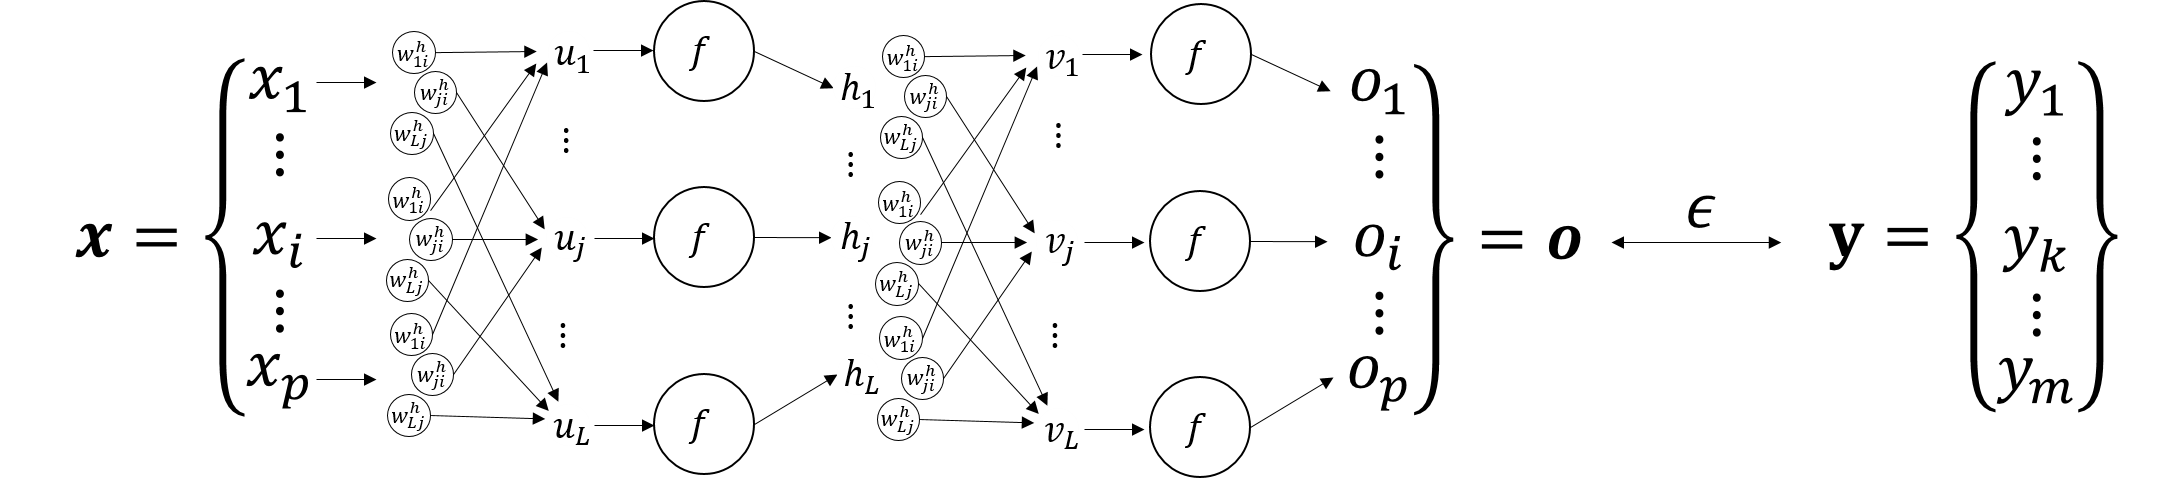
\includegraphics[width=1\linewidth]{Images/Diagrams/NeuralNetwork}
	\caption[Multilayer Perceptron]{Multilayer Perceptron}
	\label{fig:neuralnetwork}
\end{figure}

For a given input, $x$, and (expected) output, $y$, the error of the \acrshort{ann}, $ \epsilon $, is equal to the distance between the \acrshort{ann}'s outputs, $o$, and the expected outputs. The power of \acrshort{ann}s lies in the fact that they can be trained to minimize this error. 


Training the network involves firstly initialising the network with a random set of weights, $W$. A large set of training data (sets of inputs, $X$, and desired outputs, $Y$) is then presented to the network. The optimisation process (often referred to as backpropagation) proceeds by calculating the prediction error, $ \epsilon $, for each of these data sets, and then "propagating" this error value backwards through the network so that each weight can be adjusted accordingly. This is achieved by means of automatic differentiation. Automatic differentiation allows us to compute the partial derivative of the error with respect to the weights in the \acrshort{ann}, $W$ \citep{Werbos}.


This process is repeated iteratively over the training data, until the error of the \acrshort{ann} converges or some other stopping criteria is satisfied. At this point, the \acrshort{ann} will have approximated the relation, $\mathbf{X}\rightarrow \mathbf{Y}$.


A number of technical details - such as what inputs are fed into the \acrshort{ann}, what activation function is used, the number of activation functions used, the number of layers used, and the exact function used to estimate the error - have been omitted from this discussion for the sake of brevity. 

\subsection{Approximating the Calibration Function, $\mathbf{C}$} \label{subsection:neural_networks:approximating_the_calibration_function_C}
From the previous section, it follows that an \acrshort{ann} should - theoretically - be able to approximate the calibration function defined earlier, $C: f \left( D \right) \rightarrow Z$. That is, $NN \approx C$.
This can be achieved by:
\begin{enumerate}[i)]
	\itemsep0em 
	
	\item generating a set of random calibrations, $\mathbf{Z}$
	
	\item simulating a set of paths,  $\mathbf{Z}$, using the given \acrshort{sde} for every  $Z_i \in \mathbf{Z}$
	
	\item extracting a set of "inputs", $\mathbf{X}$, from the data $\mathbf{X} = f\left(\mathbf{D}\right)$
	
	\item training the \acrshort{ann} to predict the original calibrations, $\mathbf{Z}$, given the data $\mathbf{X}=f \left( \mathbf{D} \right)$ as input. This is done by setting the \acrshort{ann} to minimise the error $\epsilon$ of its output, $\mathbf{O}$ (which corresponds to an estimate of $Z_i$) and the true known values of $Z_i$.
	
	
\end{enumerate}

\begin{figure}[h]
	\centering
	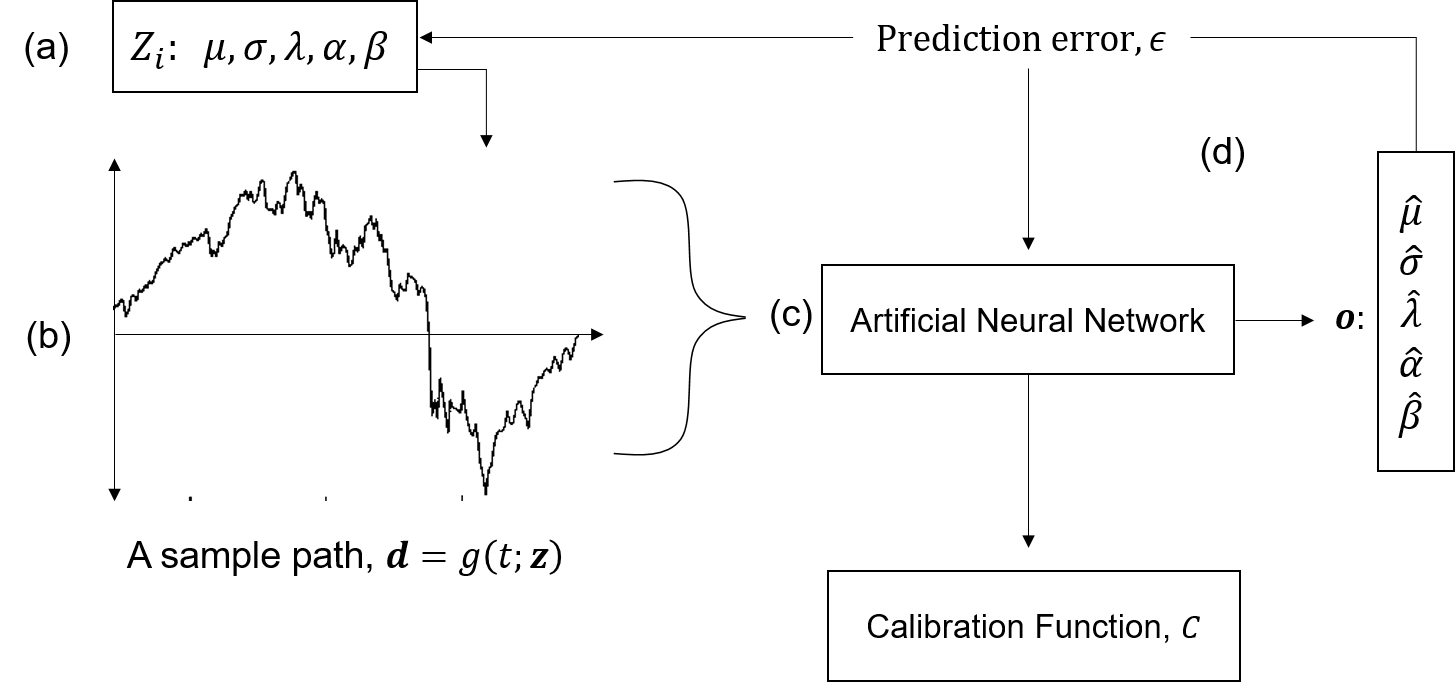
\includegraphics[width=1\linewidth]{Images/Diagrams/CalibrationSchemeDiagram}
	\caption[The Proposed Calibration Scheme]{The Proposed Calibration Scheme}
	\label{fig:calibrationschemediagram}
\end{figure}

If a large enough set of calibrations is chosen and enough data is simulated from the \acrshort{sde} using each calibration, the \acrshort{ann} will approximate the desired calibration function, $C$, for the given \acrshort{sde}.


This trained \acrshort{ann} can then be applied to real-world observations to calibrate the relevant \acrshort{sde} for the observed process.  This is done by inputting the data observed from the real-word stochastic process into the trained \acrshort{ann}. The \acrshort{ann} output, $\mathbf{o'}$, will then be an estimate of the parameters (i.e. a calibration) for the \acrshort{sde} that the \acrshort{ann} was trained on.


In this paper, the \acrshort{ann} was built and trained in Python, using Google's open source Tensorflow\texttrademark \xspace \citep{tensorflow2015-whitepaper} and Keras \citep{chollet2015keras} libraries. All model training was done using the Adam optimizer \citep{adam}.

A full list of software and packages used in this dissertation is available in appendix \ref{list_of_software_used}.

\chapter{Literature Review}
\label{chapter:literature_review}
The literature discussed throughout this research will fall into mainly two broad categories. Firstly, a review of the common methods proposed for the calibration of stochastic processes, focusing on their limitations, ease of use, universality and accuracy. Secondly, an overview of past applications of \acrshort{ann}s to modelling and model calibration. 

\section{Calibration of Stochastic Processes}
The main argument for a universal neural network approach to model calibration is that traditional methods are often unpractical. Numerous academic works substantiate this observation.


\citefullauthor{Nielsen} (\citeyear{Nielsen}) reviewed the progress made on \acrshort{sde} parameter estimation over the 80s and 90s. They note that the \acrshort{mlestimation} approach does not generalise and, having studied the \acrshort{mme} and the efficient method of moments, they explain that both of these methods will result in tests of low power due to the efficiency loss.


More recently, \citet{Mongwe} did a study on jump-diffusion processes applied to the South African equity and interest rate markets. He reported on the application and accuracy of multiple calibration methods, including the likelihood profiling approach \citep{Honore}, the standard \acrshort{mlestimation} approach, the \acrshort{mlestimation} approach and \acrfull{em}. He concluded that both \acrshort{mlestimation} and \acrshort{mme} fell short of expectations, and that the likelihood profiling and \acrshort{em} techniques worked best on parameter estimation for jump-diffusion processes (each under different restrictions on the parameters) (Mongwe, 2015). These recommendations will be applied when evaluating and comparing the performance of the neural-network calibration approach in this paper to that of existing methods.


\section{Neural Networks in Modelling and Model Calibration}
Except for the case of \citefullauthor{Xie} (\citeyear{Xie}), the task of calibrating stochastic processes using \acrshort{ann}s has not been thoroughly attempted or documented in the major academic journals examined for this research. Numerous works do however highlight the potential of \acrshort{ann}s in this field.
Multiple studies have been done on the use of \acrshort{ann}s in pricing options, and - in particular - to outperform the Black-Scholes model (\citefullauthor{Yao}; \citeyear{Yao}). The results seem to indicate that \acrshort{ann}s outperform the Black-Scholes model in volatile markets, and are particularly useful in these when the "constant $\sigma$" assumption underlying the Black-Scholes model is violated.


Tackling the issue of model calibration; \citet{Samad} investigated the application of \acrshort{ann}s to the calibration of process systems - namely that of first-order process open-loop delay identification. They concluded that \acrshort{ann}s are an attractive solution, as they do not require the subject-specific expertise vital to common engineering approaches, provide high accuracy and prove robust on real-world data.


On the topic of this paper, \citet{Xie} did an investigation into the feasibility of estimating the parameters both linear and nonlinear \acrshort{sde}s using multilayer perceptron (MLP) networks. Their investigation comprised only of small MLPs with 1-, 2- and 3-hidden-layer, fully connected architectures. They found that, under certain conditions limiting the parameter values of the process, a simple MLP would be able to estimate parameters with high accuracy ($R^2 > 0.93$). They report that this accuracy figure, however, does diminish under noisy conditions and \acrshort{sde}s with high diffusion levels. Another, often overlooked element noted by their research is the importance of the regime used to generate the simulated training data. The paper indicates to a notable increase in accuracy by using a simulation regime that makes use of the same parameters over 5 different Wiener processes, which effectively helps remove the "randomness" and noise from the dataset. They called for more research on the subject, particularly using different \acrshort{ann} architectures. What is notable about the paper presented, is that high accuracy was achieved using a simple network topology. This serves as evidence for the potential of \acrshort{ann}s to act as robust calibration estimators for \acrshort{sde}s.


\citet{Giebel} proposed a novel calibration method for time series that dynamically adapts the parameters of a stochastic model by using small MLP networks (2-layer). These \acrshort{ann}s use data from the past n observations to inform an updated parameter value. They then used the updated stochastic process to forecast the time series one day ahead, while updating the parameters at each time step as they proceed through the time series. They argue that updating the parameters of the stochastic process at each time step is more realistic, due to investors often weighting recent observations as more relevant than aged data. Using this method, different weights can be assigned to data from different dates in the past. The calibration scheme proposed in this paper could potentially add great value to the technique described by Giebel and Rainer, as it would allow the periodic recalibration of more complex processes, and the incorporation of many additional parameters. 

\chapter{Methodology}
\label{chapter:methodology}

\section{Artificial Neurons}
\label{section:artificial_neurons}

In Chapter 1, \acrshort{ann}s were introduced. Figure~\ref{fig:neuralnetwork} introduces 3 types of trainable neurons: weights (denoted by $w$), biases ($u$), and activation functions ($f$). Hence, every individual neuron multiplies the set of inputs, $x_i$ by their corresponding weights $w_i$ and adds some bias, $u$ - the sum of which is then fed through an activation function $f$. The result is propagated forward in the network to the next set of neurons. Mathematically, the output of the $k$th neuron is given by:
\begin{equation}
\mathbf{o}_k = f\left(\sum_i \left[ \mathbf{w}_{ki} \mathbf{x}_i \right] + \mathbf{u}_k\right)
\end{equation}

\subsection{Activation Functions}
The activation function $f$ is used to add non-linearity to the architecture. Without it, the model would be little more than a multivariate linear model. There are a number of choices for this activation function. The most popular being \acrlong{relu}s (\acrshort{relu}s), \acrlong{elu}s (\acrshort{elu}s), logistic sigmoid- and hyperbolic tangent functions.

Prior to the work of \citefullauthor{glorot2011deep} (\citeyear{glorot2011deep}), logistic sigmoid and hyperbolic tangent functions were the commonest activation functions in neural network architectures.However, \citet{glorot2011deep} showed that \acrshort{relu}s yield better performance. \acrshort{relu}s employ the activation function:

\begin{equation}
f\left(x\right) = \max\left(0, x\right)
\end{equation}

\citefullauthor{DBLP:journals/corr/ClevertUH15} (\citeyear{DBLP:journals/corr/ClevertUH15}) introduced the "exponential linear unit", which provide even better performance than \acrshort{relu}s, both in terms of learning speed as well as generalisation potential. An \acrshort{elu} with parameter $\alpha > 0$ has activation function:

\begin{equation}
f\left(x\right)=\left\{\begin{matrix}
x & if\ \ x > 0\\ 
\alpha \left( \exp\left(x \right ) -1\right ) & if\ \ x \leq 0
\end{matrix}\right.
\end{equation}

\begin{figure}[h]
	\begin{floatrow}
		
	 \ffigbox{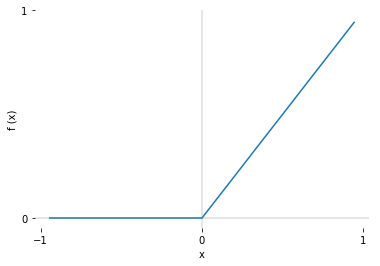
\includegraphics[width=1\linewidth]{Images/Results/relu}}{\caption[Rectifier Activation Function, f(x)]{Rectifier Activation Function (\acrshort{relu}), $f(x)$.}\label{fig:relu}}
	 
		\ffigbox{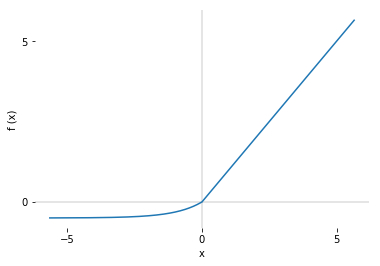
\includegraphics[width=1\linewidth]{Images/Results/elu}}{	\caption[Exponential Linear Unit (\acrshort{elu})]{Exponential Linear Unit (\acrshort{elu}) Activation Function, with $\alpha = 0.5$.}
			\label{fig:elu}}

	\end{floatrow}
\end{figure}

\section{Convolutional Layer}

Convolutional Neural Networks (\acrshort{cnn}'s) are a variation of the traditional multi-layer perceptron architecture. Like ordinary fully connected networks, they consist of neurons with trainable weights and biases. Unlike fully connected networks, these neurons are grouped into sets of small filters. With every forward pass, the filters are sequentially convolved across the extend of the input volume. This produces an activation map containing the result of the "filtration" at every point of the input volume.

In an image-recognition setting, the network will typically train filters that activate on the detection of visual features such as edges or a blotch of colour \citep{cs231n}. However, in this study, there is no definite way to ascertain what they might detect.

\begin{figure}[h]
	\centering
	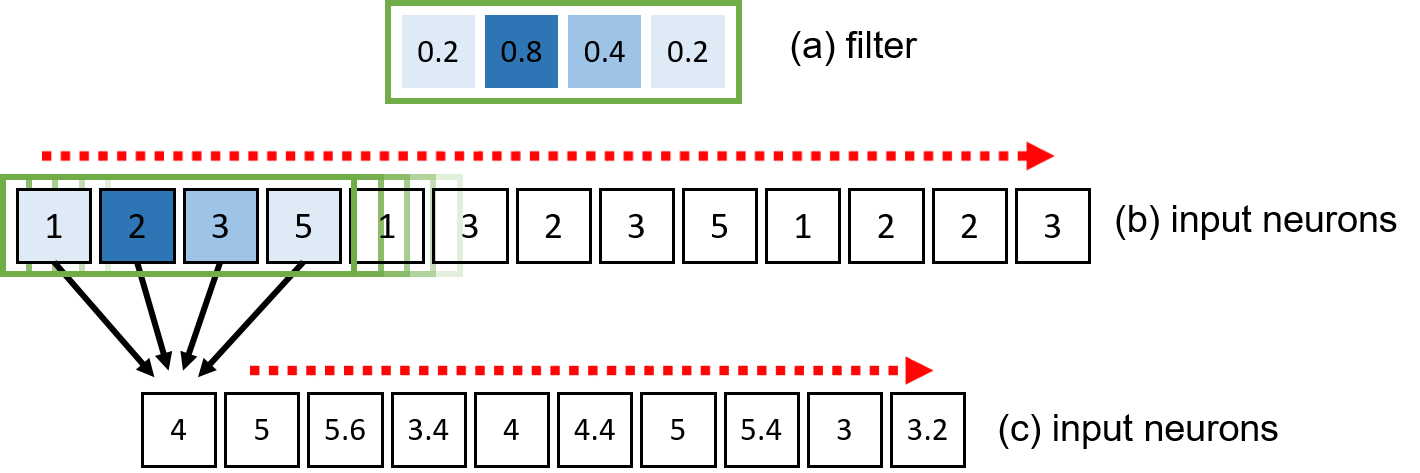
\includegraphics[width=0.9\linewidth]{Images/Diagrams/1D_Convolution}
	\caption[1D Convolutional Layer]{A One-Dimensional Convolution Layer}
	\label{fig:1dconvolution}
\end{figure}

\begin{figure}[h]
	\centering
	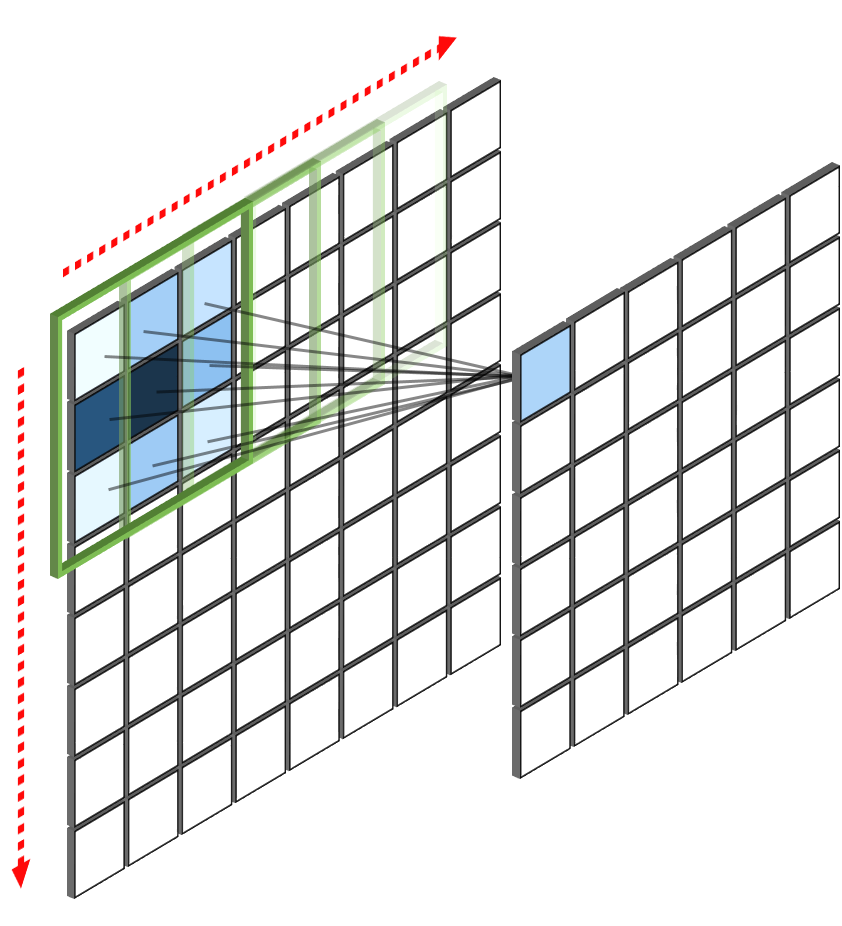
\includegraphics[width=0.4\linewidth]{Images/Diagrams/2D_Convolution}
	\caption[2D Convolution Layer]{A Two-Dimensional Convolution Layer}
	\label{fig:2dconvolution}
\end{figure}

\subsection{Pooling}
\acrshort{cnn} architectures often feature pooling layers, which aggregate the outputs of multiple preceding neurons into a single feature, which is then propagated forward through the network. Two prevalent pooling operations are subsampling (where the mean of the preceding neuron outputs are transmitted to the subsequent layer), as well as maximum pooling - which propagates the maximum output from a set of preceding neuron outputs, to the next layer. The empirical results of \citefullauthor{Scherer2010} (\citeyear{Scherer2010}) show that "a maximum pooling operation significantly outperforms subsampling operations". In the convolutional network implementations from this dissertation, extensive use was made of maximum pooling operations. Note that - unlike the filters of a convolutional layer - the weights of an average- or maximum pooling operation cannot be adjusted during training, and hence the pooling layers do not form part of the set of trainable network layers.

\begin{figure}[h]
	\centering
	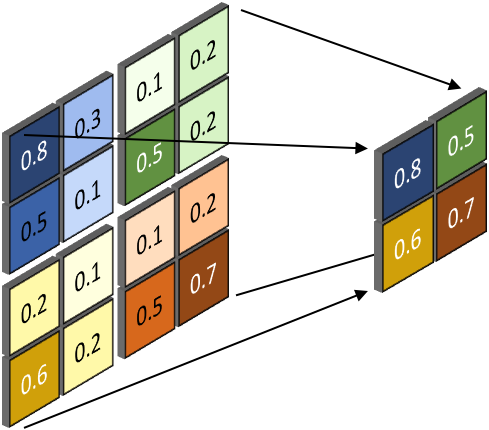
\includegraphics[width=0.4\linewidth]{Images/Diagrams/Max-Pooling_Operation}
	\caption[A $2x2$ maximum pooling operation.]{A $2x2$ maximum pooling operation.}
	\label{fig:max-poolingoperation}
\end{figure}

\section{Training Artificial Neural Networks}
Before any supervised learning approach can be utilised for inference, it needs to undergo an optimisation process known as "training". Training involves adjusting the appropriate parameters of the network (often referred to as the trainable parameters), in order to minimise the error between the output of the model, and the desired output. 
The error is defined by some selected loss function, $L$.
The artificial neurons introduced in section \ref{section:artificial_neurons} are "trained" using a technique known as backpropagation. 

\subsection{Backpropagation}
Backpropagation consists of two main steps: a propagation step and a parameter adjustment step. In turn, the propagation step consists of both forward- and backward passes. 

In the forward propagation step, the inputs are fed through the model to produce a set of output activations, $\mathbf{o'}$. These outputs are then compared to the desired outputs $\mathbf{y'}$, and an error value $\mathbf{\epsilon'}$ is obtained using some loss function $L$. That is, $\mathbf{\epsilon'} = L\left(\mathbf{o'}, \mathbf{y'}\right)$. These errors are then propagated backwards through the network to generate a set of gradients for each artificial neuron. What follows is the process of gradient descent: the gradient defines a direction (increase or decrease) as well as a magnitude in which to adjust the individual parameter (usually a weight or bias) in order to minimise the error, $\mathbf{\epsilon'}$ . In the parameter adjustment step, the trainable parameters of the model are each adjusted in the opposite direction of the gradient defined for that parameter, so as to minimise this error.

These steps are repeated until some stopping criteria is reached.

\section{Performance Measurement}
\subsection{Coefficient of Determination}
In measuring the performance of the \acrshort{ann}, we will use the the coefficient of multiple determinations, $ R^2 $, between the actual parameter values, $ \mathbf{y} $, and the \acrshort{ann}-predicted parameter values $ \mathbf{\hat{y}}$. $ R^2 $ is defined as

\begin{equation}
R^2 = 1 - \frac{\sum_{i=1}^{m}\left(y_i-\hat{y}_i\right)^2}{\sum_{i=1}^{m}\left(y_i-\overline{y}\right)^2}
\end{equation}.

where $y$ is the actual parameter value, $\hat{y}$ is the predicted parameter value, $\overline{y}$ is the mean parameter value, and $m$ is the size of the sample. Any estimate that is more accurate than the sample mean would result in an $ R^2 $ value of greater than zero. An $ R^2 $ value of 1 would indicate a perfect fit.

\subsection{Average Absolute Percentage Error}
Another model evaluation metric is the average absolute percentage error (AAPE).
\begin{equation}
AAPE = 100 \cdot \frac{1}{m} \sum_{i=1}^{m} \frac{\left| y_i - \hat{y}_i \right|}{y_i}
\end{equation}
where $y$ is the actual parameter value, $\hat{y}$ is the predicted parameter value, and $m$ is the size of the sample.

\subsection{Mean Squared Error}
A natural loss function to consider in the optimisation procedure concerned in this dissertation is that of \textit{mean squared error} (MSE). MSE measures the squared mean deviation of the predicted values (yielded by the model under consideration) from the actual observed values.
\begin{equation}
MSE = \sum_{i=1}^{m}\left(y_i-\hat{y}_i\right)^2
\end{equation}
where $y$ is the actual observed parameter (output) value, $\hat{y}$ is the predicted parameter (output) value, and $m$ is the size of the sample.

\chapter{Simulation Study}
\label{chapter:simulation_study}

It is important to note that when building a neural network for a specific modelling exercise, one has little prior knowledge of what the model should look like. Rough guidlines do exist, for example that \acrfull{rnn} architectures are often used for time series problems \citep{Karpathy} or that \acrlong{cnn}s (\acrshort{cnn}s) are well suited to image recognition tasks \citep{LISALab}. Beyond these vague guidelines however, little evidence exists to inform the potential properties that a network might need.

\section{The Merton Jump-Diffusion Stochastic Process}

The Merton Jump-Diffusion stochastic process, presented in the seminal work of \citet{Merton}, aimed to address the limitations of the \acrshort{gbm} process. It has the stochastic differential equation,

\begin{equation}
d S_t =  \mu S_t dt  +\sigma S_t dW_t + S_t dJ_t 
\end{equation}
where
\begin{equation}
J_t = \sum_{j=1}^{N_t}(V_j - 1)
\end{equation}

is a compound Poisson process. $V_j$ are independent, identically distributed positive random variables representing the jump sizes. $N_t, t \geq 0$ is a Poisson process with intensity $\lambda$, which is independent of $J_t$ and $W_t$.

To obtain the log returns, we can derive the function $f(t, S_t) = \ln{S_t}$ using It\^{o}'s formula:

\begin{equation} \label{equation:merton_log_returns}
d\ln{S_t} = \frac{1}{S_t}dS_t - \frac{1}{2{S_t}^2}\left(dS_t\right)^2 = \left( \mu - \frac{\sigma^2}{2} \right)dt +\sigma dW_t + dJ_t 
\end{equation}

In this dissertation we will have $V_j$ follow a log-normal distribution with parameters $\mu_{jumps}$ and $\sigma_{jumps}$.

\subsection{The Parameters}

To better understand the effects of the parameters ($\mu$, $\sigma$, $\lambda$, $\mu_{jumps}$ and $\sigma_{jumps}$) on the resulting process, it is important to note that the Merton Jump-Diffusion process can effectively be separated into two distinct components: the diffusion process (\acrshort{gbm}), as well as a jumps process. This is illustrated in figure \ref{fig:merton_jd_components} below.

\begin{figure}[h]
	\centering
	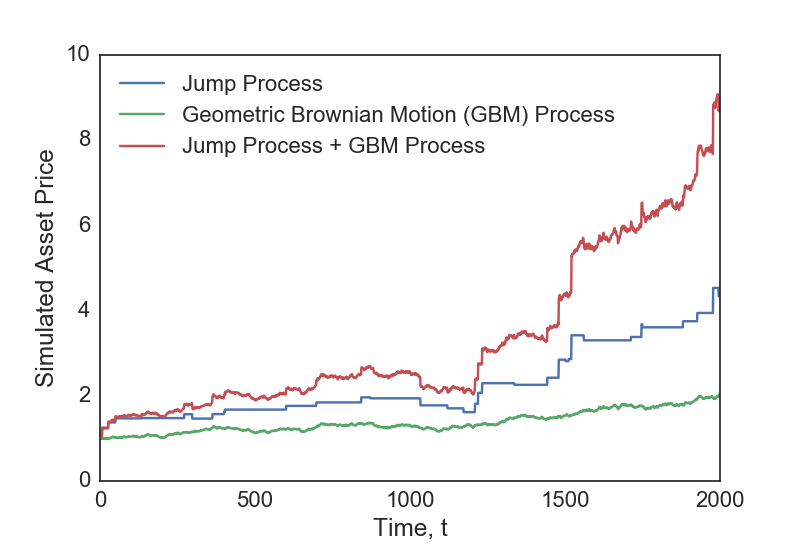
\includegraphics[width=0.7\linewidth]{Images/Parameter-Effects/Merton_JD_Components}
	\caption[The components of a simulated path from the Merton Jump-Diffusion process]{The simulated asset price resulting from a Merton Jump-Diffusion returns process, as well as that of its two components: a jumps process, and a \acrshort{gbm} process.}
	\label{fig:merton_jd_components}
\end{figure}

\subsubsection{Mu $\left(\mu\right)$ and sigma $\left(\sigma\right)$}

Both mu $\left(\mu\right)$ and sigma $\left(\sigma\right)$ form part of the \acrshort{gbm} component of the process: $\mu$ defines the mean returns yielded from the process, while $\sigma$ specifies the volatility of the returns. The effects of these parameters on the process are illustrated in figures \ref{fig:effects_mu} and \ref{fig:effects_sigma} in appendix \ref{appendix:merton_jd_parameters_effects}.

\subsubsection{Lambda $\left(\lambda\right)$, jumps mu $\left(\mu_{jumps}\right)$ and jumps sigma $\left(\sigma_{jumps}\right)$}

Lambda $\left(\lambda\right)$, jumps mu $\left(\mu_{jumps}\right)$ and jumps sigma $\left(\sigma_{jumps}\right)$ form part of the jump-process. Lambda $\left(\lambda\right)$ is the intensity parameter of the Poisson process, $N_t$, and hence defines the probability that a jump might occur at any given time. The jumps are drawn from a normal distribution with parameters $\mu_{jumps}$ and $\sigma_{jumps}$. These parameters hence define the mean and deviation of the jump sizes respectively. The effects of these parameters on the process are illustrated in figures \ref{fig:effects_lambda}, \ref{fig:effects_jumps_mu} and \ref{fig:effects_jumps_sigma} in appendix \ref{appendix:merton_jd_parameters_effects}.

\subsection{Simulation}
The neural network models will be trained on the log-returns of the simulated processes. These processes will be simulated using a random set of parameters (within certain bounds).

The simulated parameters, $\mu$, $\sigma$, $\lambda$, $\mu_{jumps}$ and $\sigma_{jumps}$ will be constrained to the following bounds: $\mu \in [-1, 1]$, $\sigma \in [0.001, 0.2]$, $\lambda\in [0.0001, 0.025]$, $\sigma_{jumps} \in [0.001, 0.2]$, and $\mu_{jumps}\in [-0.5, 0.5]$.

\section{Fully Connected Neural Network}

\subsection{Multiple Parameter Prediction Architecture} \label{subsection:fully_connected_ff_nn:architecture}
The first study was done on a standard 9-layer fully connected multi-perceptron architecture, trained to predict all five parameters of the Merton Jump-Diffusion process at once.

\begin{figure}[h]
	\centering
	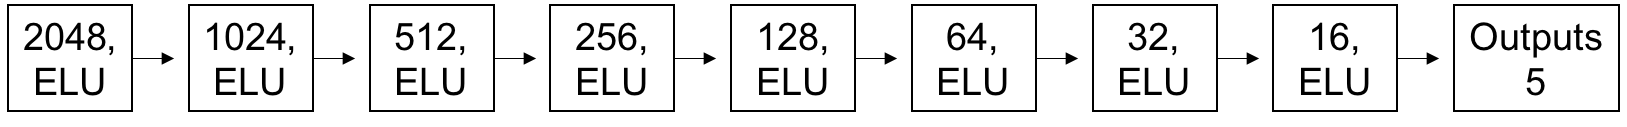
\includegraphics[width=1\linewidth]{Images/Diagrams/Network-Structures/MultipleOutputFullyConnectedANN}
	\caption[Multiple Output Prediction \acrshort{ann}]{9-Layer Fully Connected Feed-forward \acrshort{ann}}
	\label{fig:multipleoutputcnn}
\end{figure}

The experiments were performed using \acrshort{elu} activation functions in the network. 

\subsection{The Dataset}

The dataset on which the Fully Connected \acrshort{ann} was trained, was created using the following steps:
\begin{enumerate}[1)]
	\itemsep0em 
	\item  Random sets of parameters, $\mathbf{z}_i$, with ($\mu \in \left[-1, 1\right]$, $\sigma \in \left[0.001, 0.2\right]$, $\lambda \in \left(0, 0.025\right]$, $\mu_{jumps} \in \left[-0.5, 0.5\right]$ and $\sigma_{jumps} \in \left[0.001, 0.2\right])$ were uniformly generated.
	\item  The daily log returns from a Merton Jump-Diffusion stochastic process (equation \ref{equation:merton_log_returns}) were simulated using these randomly generated parameter sets, $\mathbf{z}_i$, as parameters.
	\item  For each set of returns, the first 20 sample moments, as well as the autocorrelations up to the first 40 lags were calculated.
	\item For every parameter set, its corresponding set of moments and autocorrelations were fed into the input layer of the \acrshort{ann} described in subsection \ref{subsection:fully_connected_ff_nn:architecture} above. The \acrshort{ann} was then trained, using the process of backpropagation, to produce an estimate, $\mathbf{o}_i$, of the original set of parameters, $\mathbf{z}_i$. This was done by minimizing the mean squared error between the vectors $\mathbf{z}_i$ and $\mathbf{o}_i$ (see the diagram in figure \ref{fig:calibrationschemediagram}).
\end{enumerate}

\subsection{Training}
\begin{figure}[h]
	\ffigbox{
		\begin{subfloatrow}
			
			\ffigbox{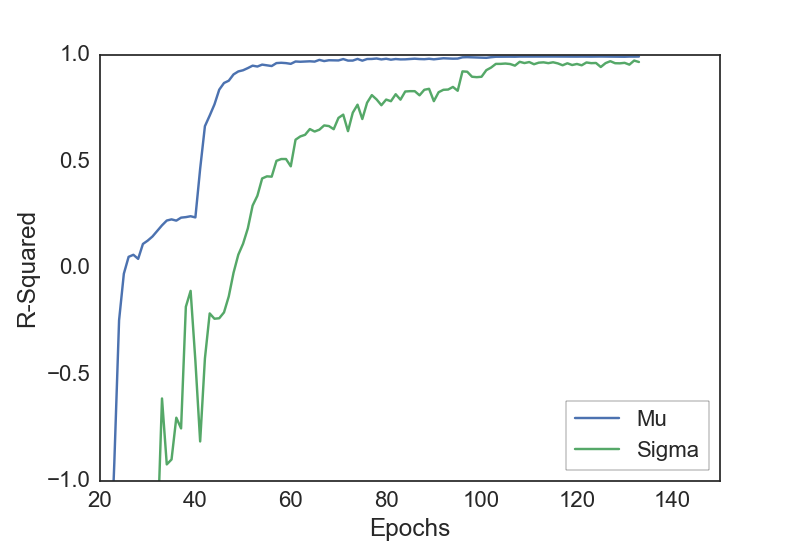
\includegraphics[width=1.06\linewidth]{Images/Prediction-Convergence/FullyConnectedNN-MultipleOutput-ELU/training_r2_values_mu_sigma}}{
				\caption[]{$\sigma,  \mu$}
				\label{fig:training:fully_connected_mu_and_sigma}}
			
			\ffigbox{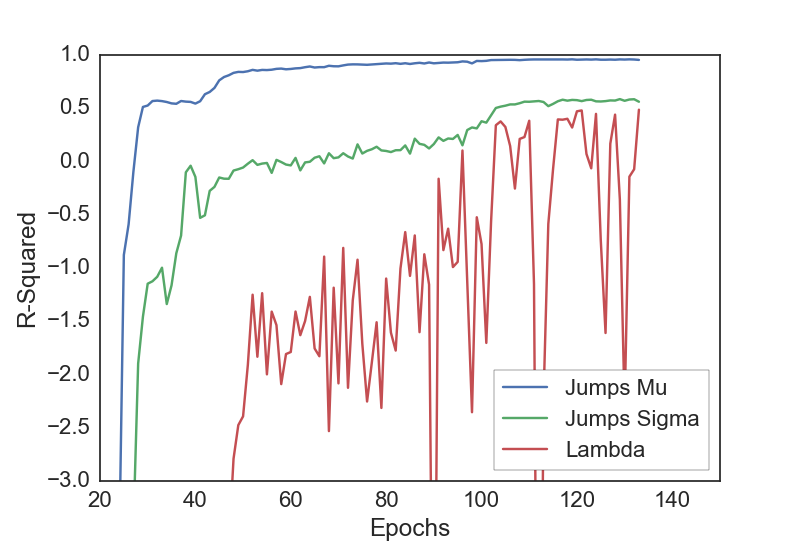
\includegraphics[width=1\linewidth]{Images/Prediction-Convergence/FullyConnectedNN-MultipleOutput-ELU/training_r2_values_jumps}}{
				\caption[]{$\lambda$, $\sigma_{jumps}$, $\mu_{jumps}$}
				\label{fig:training:fully_connected_jumps}}
			
		\end{subfloatrow}
	}{
		
		\caption{R-Squared values over the training process for the multiple parameter prediction fully connected architecture (\acrshort{elu} activation units).}}
\end{figure}

Figures \ref{fig:training:fully_connected_mu_and_sigma} and \ref{fig:training:fully_connected_jumps} illustrate the R-Squared values throughout the training process of the fully connected architecture.

\section{Convolutional Neural Network}

\subsection{Multiple Parameter Prediction Architecture}
\label{chap:ConvolutionalNeuralNetwork-section:MultipleParameterPredictionArchitecture}
The second study was done on a fairly standard 8-layer convolutional architecture, which produced estimates for all five parameters.

\begin{figure}[h]
	\centering
	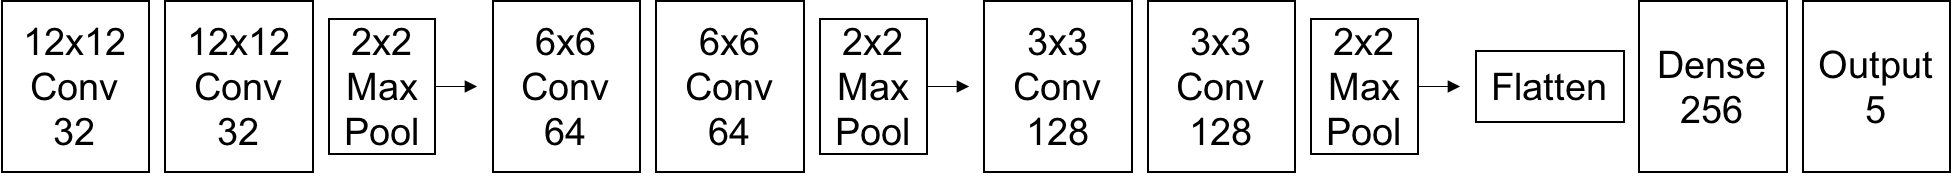
\includegraphics[width=1\linewidth]{Images/Diagrams/Network-Structures/MultipleOutputCNN}
	\caption[Multiple Output Prediction \acrshort{cnn}]{8-Layer \acrshort{cnn}}
	\label{fig:multipleoutputcnn}
\end{figure}

Experiments were performed using \acrshort{elu} activation functions. 

\begin{figure}[h]
	\centering
	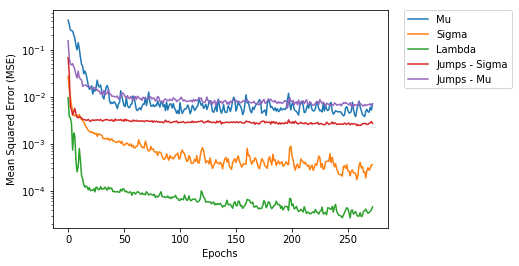
\includegraphics[width=0.7\linewidth]{Images/Results/Training/COVNET_MO_MSE}
	\caption[MSE values over the training process for the 8-Layer \acrshort{cnn}]{MSE values over the training process for the multiple parameter prediction convolutional architecture. Each epoch involves 10 iterations of a simulated batch of 150 randomly selected process parameters.}
	\label{fig:covnetmomse}
\end{figure}

The reasons for the large difference in MSE values are related to the nature of the parameters. For example Mu ($\mu$) - the drift of the \acrshort{gbm} component of the process - can take on values between $-0.5$ and $0.5$, while Lambda ($\lambda_{jumps}$) - the probability of a jump occurring at any given point, can only take on values between $0$ and $0.003$.

\begin{figure}[h]
	\ffigbox{
		\begin{subfloatrow}
			
			\ffigbox{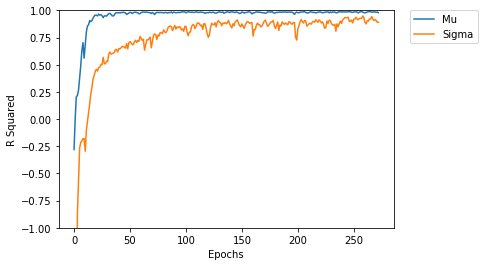
\includegraphics[width=1\linewidth]{Images/Results/Training/COVNET_MO_R2_}}{
				\caption[]{$\sigma,  \mu$}
				\label{fig:covnetmor2}}
			
			\ffigbox{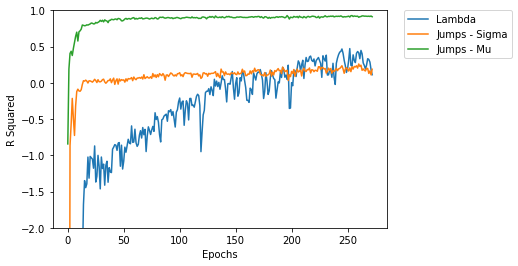
\includegraphics[width=1.06\linewidth]{Images/Results/Training/COVNET_MO_R2_2}}{
				\caption[]{$\lambda$, $\sigma_{jumps}$, $\mu_{jumps}$}
				\label{fig:covnetmor22}}
			
		\end{subfloatrow}
		}{
		
		\caption{R-Squared values over the training process for the multiple parameter prediction convolutional architecture (\acrshort{elu} activation units).}}
\end{figure}

\subsection{Dedicated Single Parameter Prediction Architecture}
\label{chap:ConvolutionalNeuralNetwork-section:SingleParameterPredictionArchitecture}
In training the multiple output model, one might notice a slight oscillation in the accuracy of the parameters. At higher levels of accuracy, as the network becomes more accurate at predicting one output, it might become less accurate for another. There seems to exist a payoff, whereby the accuracy reduces as the prediction accuracy for another increases.

This raises the question of a dedicated network architecture for every parameter. A slight variation on the architecture used in \ref{chap:ConvolutionalNeuralNetwork-section:MultipleParameterPredictionArchitecture} above was implemented. The structure was scaled down to six trainable layers, with a larger penultimate layer. The architecture only outputs an estimate for a single parameter. Hence, using this architecture, separate networks will be used to individually estimate the values of each of the parameters, $\mu$, $\sigma$, $\lambda$, $\mu_{jumps}$ and $\sigma_{jumps}$.

\begin{figure}[h]
	\centering
	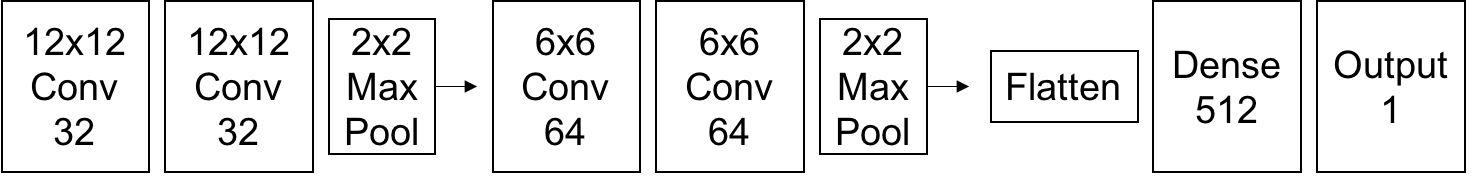
\includegraphics[width=0.75\linewidth]{Images/Diagrams/Network-Structures/SingleParameterDedicatedCNN}
	\caption[Dedicated Single Parameter Prediction \acrshort{cnn}]{6-Layer \acrshort{cnn}}
	\label{fig:singleparameterdedicatedcnn}
\end{figure}

The following sections will discuss the convergence of the dedicated models in comparison to the multiple output prediction model. The final prediction accuracy of the model will be discussed in Chapter \ref{chapter:results}.

\subsubsection{Lambda}

The most obvious parameter estimation issue in the multiple output model of \ref{chap:ConvolutionalNeuralNetwork-section:MultipleParameterPredictionArchitecture}, exists with $\lambda$, which - as clearly visible in figure \ref{fig:covnetmor22} - exhibits a reluctance to converge to a desired level of accuracy. The dedicated single architecture defined in figure \ref{fig:singleparameterdedicatedcnn} was implemented and trained to predict only the single parameter value $\lambda$ per sample path. 

\begin{figure}[h]
	\centering
	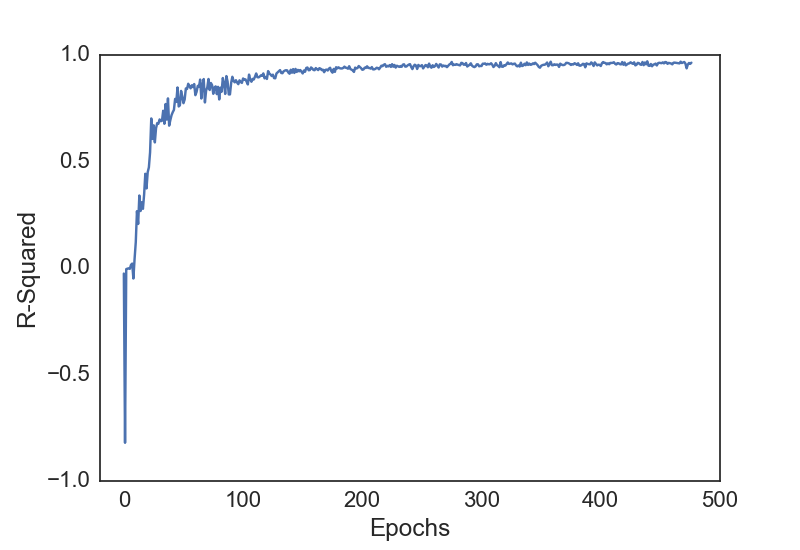
\includegraphics[width=0.5\linewidth]{Images/Prediction-Convergence/ConvolutionalNN-SingleOutput/Lambda-RSquared}
	\caption[R-Squared values for the predictions of $\lambda$ over the training process for the single parameter prediction convolutional architecture (\acrshort{elu} activation units).]{R-Squared values for the estimates of $\lambda$ over the training process for the single parameter prediction convolutional architecture (\acrshort{elu} activation units).}
	\label{fig:lambda-rsquared}
\end{figure}

The result is a much quicker and smoother convergence to an acceptable level of accuracy, as visible in figure \ref{fig:lambda-rsquared}. Compare this to the very rough convergence of $\lambda$ in figure \ref{fig:covnetmor22}. Quicker convergence leads to less training time and ultimately easier use of the model.

\section{Sensitivity Tests}
Due to the nature of the parameters involved in the Merton Jump-Diffusion process, one could expect interactions between parameter estimates. For example, increasing the $\mu_{jumps}$ parameter might cause "confusion", since a model could "interpret" larger jumps as a higher rate of volatility from the \acrshort{gbm} $\sigma$ component, and hence produce higher values of $\sigma$. What follows is an investigation into how sensitive the individual parameter estimates are with respect to changes in the magnitudes of the other parameters. 

This investigation was performed using $1000$ simulated sample paths from a Merton Jump-Diffusion process with parameters $\mu, \sigma, \lambda, \mu_{jumps}$ and $\sigma_{jumps}$. With each test, a single parameter was selected to be varied during the training process. The effect of this parameter change on the \acrshort{ann} performance was then monitored by reading the estimates of each of the other parameters and comparing them to their actual values.

\subsubsection{Variations in $\mu$}
%\begin{figure}[h]
%	\centering
%	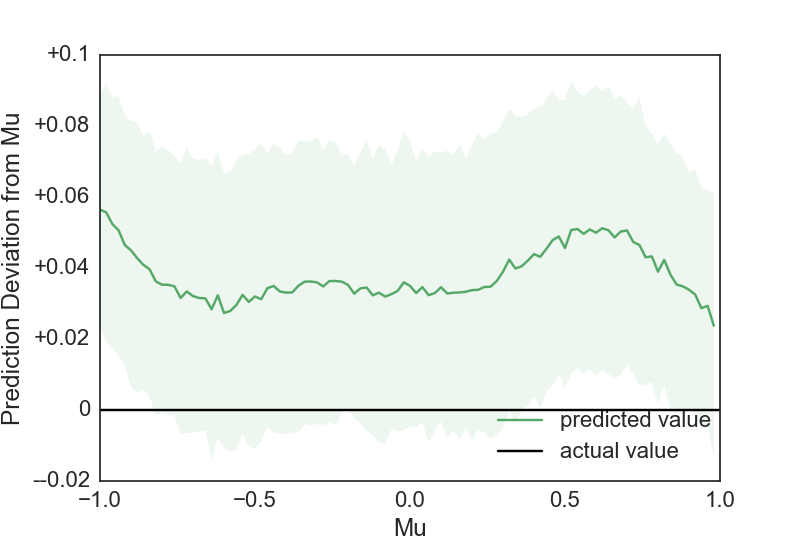
\includegraphics[width=0.7\linewidth]{Images/Output-Sensitivity-Results/ConvolutionalNN-MultipleOutput-ELU/Varying-Mu/Mu}
%	\caption{The deviation (with $68\%$ confidence interval) of the $\hat{\mu}$ parameter estimate from the actual parameter value, $\mu$, for different values of $\mu$. All the other parameters are kept constant as $\sigma = 0.1, \lambda = 0.02, \mu_{jumps} = 0.05$ and $\sigma_{jumps} = 0.07$}
%	\label{fig:sensitivity_test:multiple_output:varying_mu:mu}
%\end{figure}

\begin{figure}[h]
	\ffigbox{
%		\begin{subfloatrow}
%			
%			\ffigbox{
%				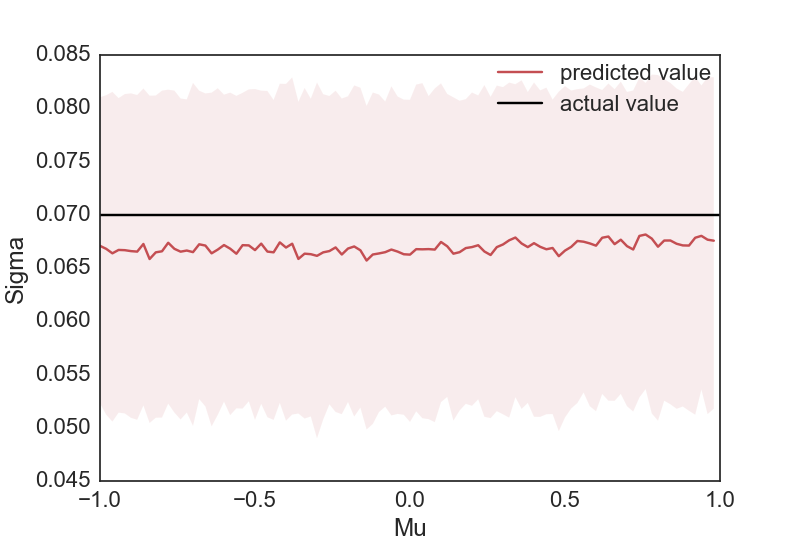
\includegraphics[width=1\linewidth]{Images/Output-Sensitivity-Results/ConvolutionalNN-MultipleOutput-ELU/Varying-Mu/sigma}
%			}{
%				\caption{The $\hat{\sigma}$ parameter estimate plotted against the actual parameter value, $\sigma = 0.1$, for different values of $\mu$.}
%				\label{fig:sensitivity_test:multiple_output:varying_mu:sigma}
%			}
%		
%			\ffigbox{
%			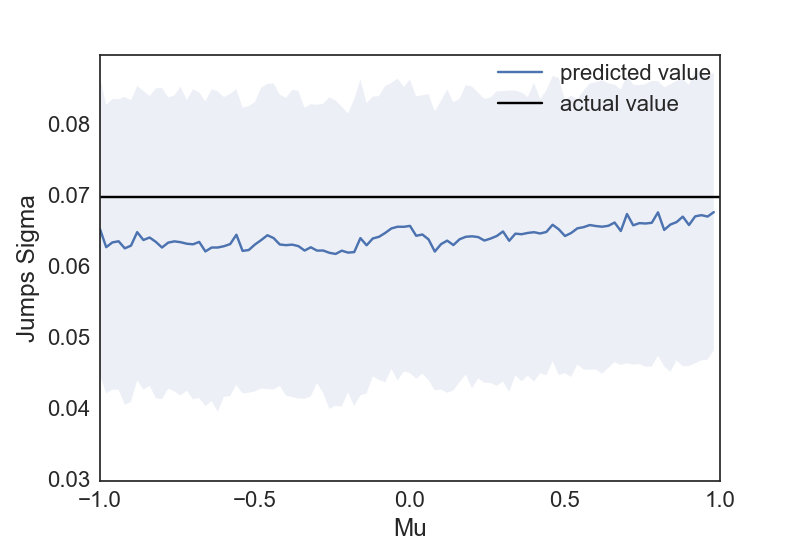
\includegraphics[width=1\linewidth]{Images/Output-Sensitivity-Results/ConvolutionalNN-MultipleOutput-ELU/Varying-Mu/Jumps_Sigma}
%			}{
%			\caption{The $\hat{\sigma}_{jumps}$ parameter estimate plotted against the actual parameter value, $\sigma_{jumps} = 0.07$, for different values of $\mu$.}
%			\label{fig:sensitivity_test:multiple_output:varying_mu:jumps_sigma}
%			}
%
%		\end{subfloatrow}
		\begin{subfloatrow}
			
			\ffigbox{	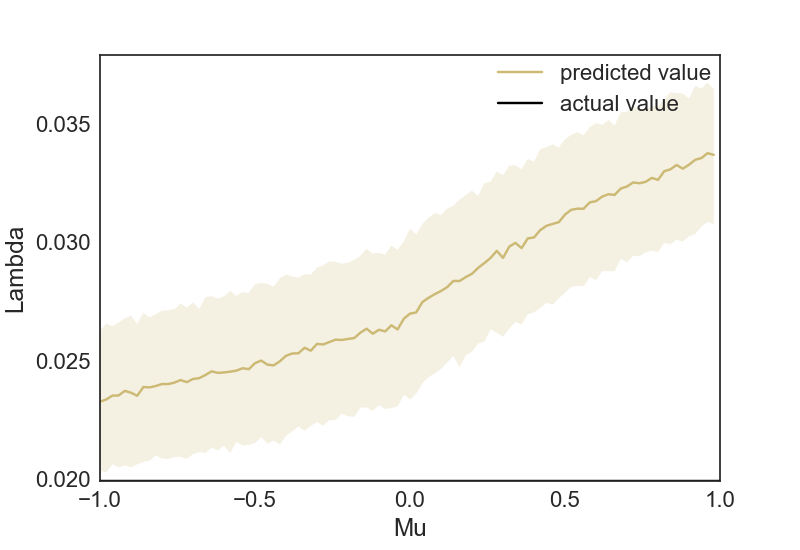
\includegraphics[width=1\linewidth]{Images/Output-Sensitivity-Results/ConvolutionalNN-MultipleOutput-ELU/Varying-Mu/Lambda}
			}{
				\caption{The $\lambda$ parameter estimate plotted against the actual parameter value, $\lambda = 0.02$, for different values of $\mu$.}
				\label{fig:sensitivity_test:multiple_output:varying_mu:lambda}
			}
			
			\ffigbox{
				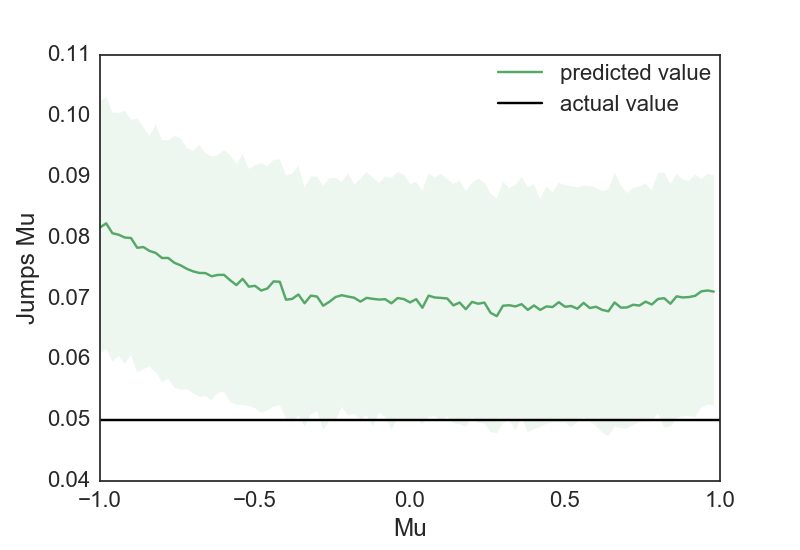
\includegraphics[width=1\linewidth]{Images/Output-Sensitivity-Results/ConvolutionalNN-MultipleOutput-ELU/Varying-Mu/Jumps_Mu}
			}{
				\caption{The $\hat{\mu}_{jumps}$ parameter estimate plotted against the actual parameter value, $\mu_{jumps} = 0.05$, for different values of $\mu$.}
				\label{fig:sensitivity_test:multiple_output:varying_mu:jumps_mu}
			}
	\end{subfloatrow}}{
		\caption{The parameter estimates (with $68\%$ confidence interval) of $\hat{\sigma}$, $\hat{\lambda}$, $\hat{\mu}_{jumps}$ and $\hat{\sigma}_{jumps}$, plotted against their actual values ($\sigma = 0.1$, $\lambda = 0.02$, $\mu_{jumps} = 0.05$ and $\sigma_{jumps} = 0.07$), while varying the $\mu$ parameter in the range $\left(-1.0, 1.0\right)$.}
		\label{fig:sensitivity_test:multiple_output:varying_mu}}
\end{figure}
Of all the parameters involved in the Merton Jump-Diffusion process, $\mu$ arguably has the least interaction with the estimates of the other parameters. 

It is rather strange that the model exhibits a tendency to consistently underestimate the value of $\lambda$ (Figure \ref{fig:sensitivity_test:multiple_output:varying_mu:lambda}). This is clear throughout the investigation - $\lambda$ is almost always underestimated. This is not something to be expected, since \acrshort{ann}s have the property of easily being able to correct for bias.
Similarly, all other parameters (besides $\mu$) kept constant, the model seems to consistently overestimate the value of $\mu_{jump}$ (Figure \ref{fig:sensitivity_test:multiple_output:varying_mu:jumps_mu}). As with the estimate of $\lambda$, one would expect and \acrshort{ann} to be able to easily correct for this clear bias.

\subsubsection{Variations in $\sigma$}

\begin{figure}[h]
	\centering
	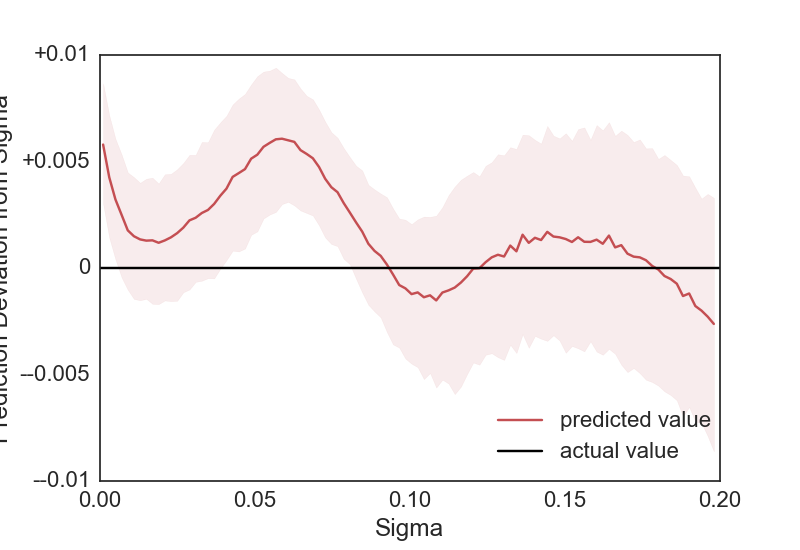
\includegraphics[width=0.5\linewidth]{Images/Output-Sensitivity-Results/ConvolutionalNN-MultipleOutput-ELU/Varying-Sigma/Sigma}
	\caption{The deviation (with $68\%$ confidence interval) of the $\hat{\sigma}$ parameter estimate from the actual parameter value, $\sigma$, for different values of $\sigma$. All the other parameters are kept constant as $\mu = 0.05, \lambda = 0.02, \mu_{jumps} = 0.05$ and $\sigma_{jumps} = 0.07$.}
	\label{fig:sensitivity_test:multiple_output:varying_sigma:sigma}
\end{figure}

As to be expected, larger volatility tends to widen the confidence interval around a particular parameter estimate. This is particularly clear in figure \ref{fig:sensitivity_test:multiple_output:varying_sigma:sigma}, where the confidence regarding the estimate of $\hat{\sigma}$ falls, as $\sigma$ increases.
The most clear-cut illustration of this can be seen in the estimates of $\hat{\mu}$ in figure \ref{fig:sensitivity_test:multiple_output:varying_sigma:mu}, where there is a clearly visible widening of the confidence interval as sigma increases.

\begin{figure}[h]
	\ffigbox{
		\begin{subfloatrow}
			
			\ffigbox{
				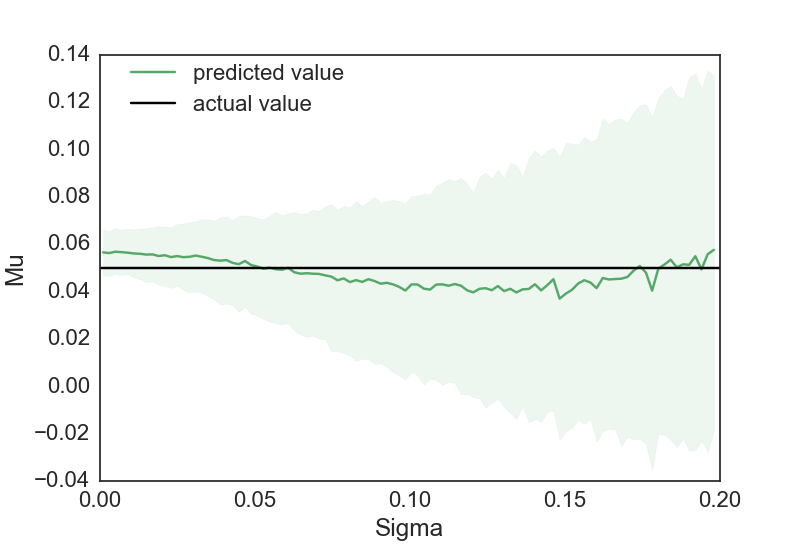
\includegraphics[width=1\linewidth]{Images/Output-Sensitivity-Results/ConvolutionalNN-MultipleOutput-ELU/Varying-Sigma/Mu}
			}{
				\caption{The mean $\hat{\mu}$ parameter estimate plotted against the actual parameter value, $\mu = 0.05$, for different values of $\sigma$.}
				\label{fig:sensitivity_test:multiple_output:varying_sigma:mu}
			}
			
			\ffigbox{	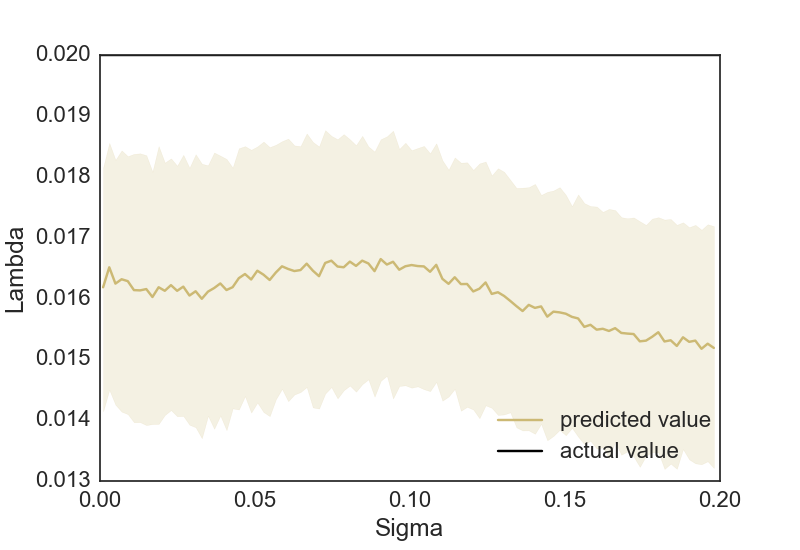
\includegraphics[width=1\linewidth]{Images/Output-Sensitivity-Results/ConvolutionalNN-MultipleOutput-ELU/Varying-Sigma/Lambda}
			}{
				\caption{The mean $\lambda$ parameter estimate plotted against the actual parameter value, $\lambda = 0.02$, for different values of $\sigma$.}
				\label{fig:sensitivity_test:multiple_output:varying_sigma:lambda}
			}
			
		\end{subfloatrow}
%		\begin{subfloatrow}
%			
%			\ffigbox{
%				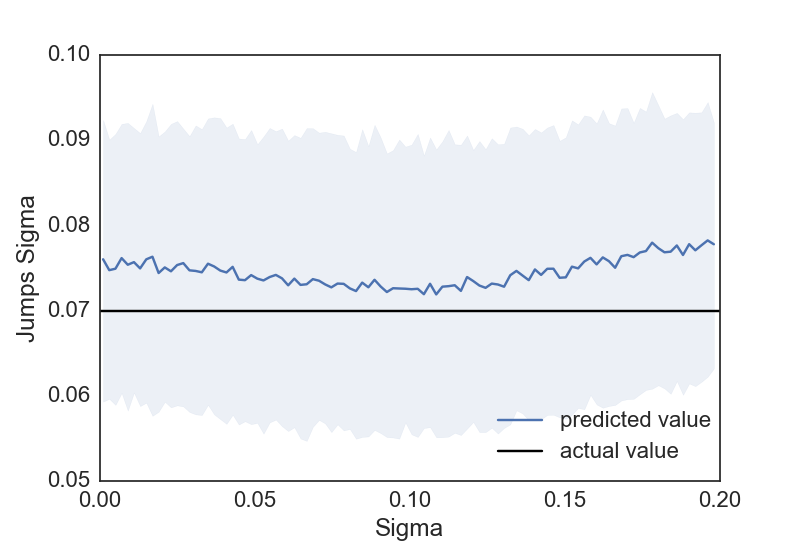
\includegraphics[width=1\linewidth]{Images/Output-Sensitivity-Results/ConvolutionalNN-MultipleOutput-ELU/Varying-Sigma/Jumps_Sigma}
%			}{
%				\caption{The mean $\hat{\sigma}_{jumps}$ parameter estimate plotted against the actual parameter value, $\sigma_{jumps} = 0.07$, for different values of $\sigma$.}
%				\label{fig:sensitivity_test:multiple_output:varying_sigma:jumps_sigma}
%			}
%			
%			\ffigbox{
%				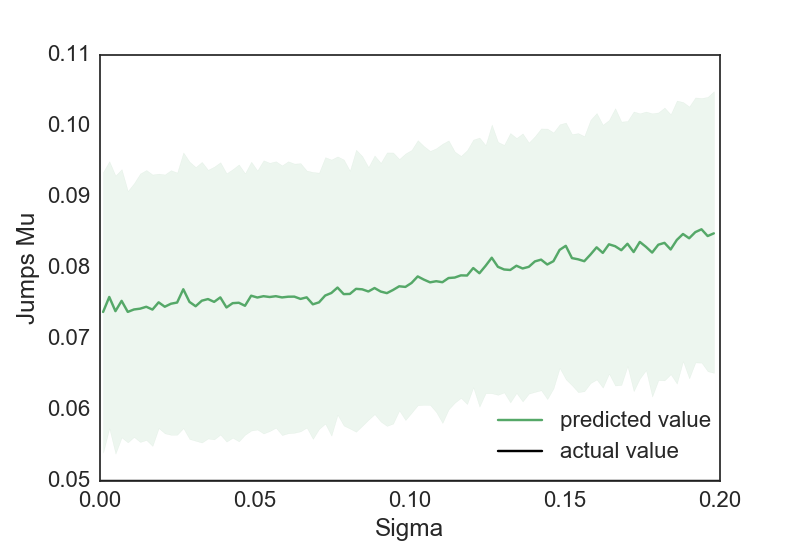
\includegraphics[width=1\linewidth]{Images/Output-Sensitivity-Results/ConvolutionalNN-MultipleOutput-ELU/Varying-Sigma/Jumps_Mu}
%			}{
%				\caption{The mean $\hat{\mu}_{jumps}$ parameter estimate plotted against the actual parameter value, $\mu_{jumps} = 0.05$, for different values of $\sigma$.}
%				\label{fig:sensitivity_test:multiple_output:varying_sigma:jumps_mu}
%			}
%	\end{subfloatrow}
		}{
		\caption{The mean parameter estimates (with $68\%$ confidence interval) of $\hat{\mu}$, $\hat{\lambda}$, $\hat{\mu}_{jumps}$ and $\hat{\sigma}_{jumps}$, plotted against their actual values ($\mu = 0.05$, $\lambda = 0.02$, $\mu_{jumps} = 0.05$ and $\sigma_{jumps} = 0.07$), while varying the $\sigma$ parameter in the range $\left(0, 0.2\right)$.}
		\label{fig:sensitivity_test:multiple_output:varying_sigma}}
\end{figure}

%The effect of larger volatility in the \acrshort{gbm} process also has a slight upward push on the estimate of $\mu_{jumps}$ (Figure \ref{fig:sensitivity_test:multiple_output:varying_sigma:jumps_mu}). This is to be expected, as larger volatility could conceivably be interpreted as larger jumps. 

%The \acrshort{ann} seems to exhibit the ability to distinguish between the volatility of the \acrshort{gbm} process ($\sigma$) and that of the jumps process ($\sigma_{jumps}$). This is clear from figure \ref{fig:sensitivity_test:multiple_output:varying_sigma:jumps_sigma}, as the value of $\sigma$ seems to put little pressure on the estimate of $\sigma_{jumps}$.

%The models seems to produce a consistent underestimate for the value of $\lambda$, and a consistent overestimate for the value of $\mu_{jumps}$.

\subsubsection{Variations in $\lambda$}

\begin{figure}[h]
	\centering
	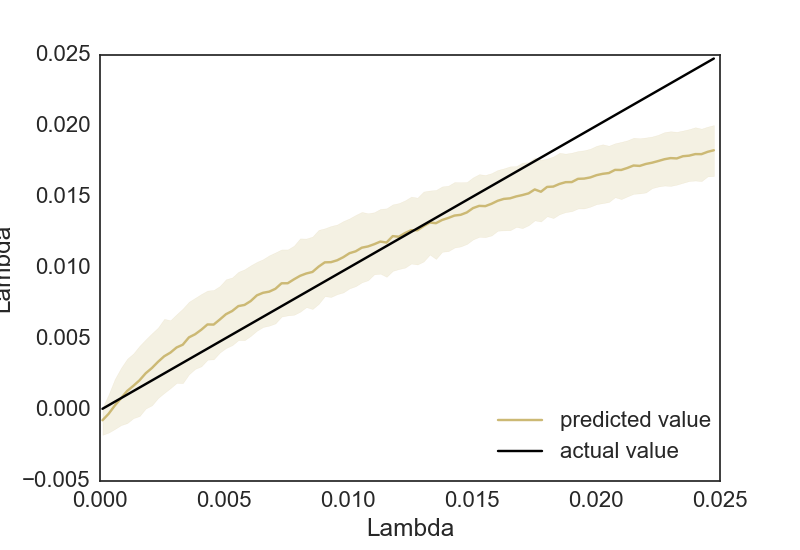
\includegraphics[width=0.5\linewidth]{Images/Output-Sensitivity-Results/ConvolutionalNN-MultipleOutput-ELU/Varying-Lambda/Lambda}
	\caption{The mean deviation (with $68\%$ confidence interval) of the $\hat{\lambda}$ parameter estimate from the actual parameter value, $\lambda$, for different values of $\lambda$. All the other parameters are kept constant as $\mu = 0.05, \sigma = 0.1, \mu_{jumps} = 0.05$ and $\sigma_{jumps} = 0.07$.}
	\label{fig:sensitivity_test:multiple_output:varying_lambda:lambda}
\end{figure}

The multiple output prediction model shows a slight overestimation of $\hat{\lambda}$ for small values of $\lambda$, and a slight underestimation for larger values of $\lambda$ (Figure \ref{fig:sensitivity_test:multiple_output:varying_lambda:lambda})

Figure \ref{fig:sensitivity_test:multiple_output:varying_lambda:jumps_sigma} shows an interesting relationship between the value of $\hat{\sigma}_{jumps}$ and $\lambda$. The model estimate of $\hat{\sigma}_{jumps}$ shows an inversely proportional relationship to the value of $\lambda$. Larger $\lambda$ also seems to make the model "less confident" in it's estimate of $\sigma_{jumps}$.

In figure \ref{fig:sensitivity_test:multiple_output:varying_lambda:jumps_mu}, we see that the opposite is true for the estimate of $\hat{\mu}_{jumps}$. As might be expected, small $\lambda$ values tend to suffocate the estimate of $\hat{\mu}_{jumps}$. It is conceivable that lower values of $\lambda$ might result in less jumps, which could be "misinterpreted" as a lower mean jump size.

\begin{figure}[h]
	\ffigbox{
%		\begin{subfloatrow}
%			
%			\ffigbox{
%				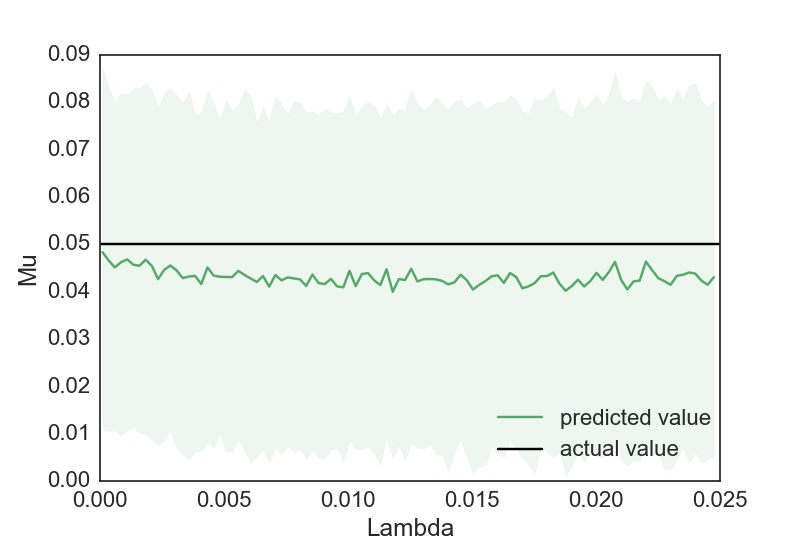
\includegraphics[width=1\linewidth]{Images/Output-Sensitivity-Results/ConvolutionalNN-MultipleOutput-ELU/Varying-Lambda/Mu}
%			}{
%				\caption{The mean $\hat{\mu}$ parameter estimate plotted against the actual parameter value, $\mu = 0.05$, for different values of $\lambda$.}
%				\label{fig:sensitivity_test:multiple_output:varying_lambda:mu}
%			}
%			
%			\ffigbox{	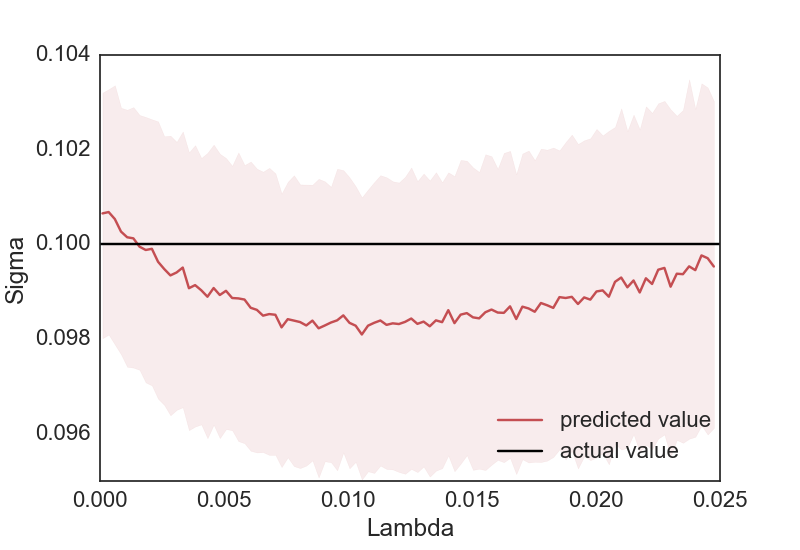
\includegraphics[width=1\linewidth]{Images/Output-Sensitivity-Results/ConvolutionalNN-MultipleOutput-ELU/Varying-Lambda/Sigma}
%			}{
%				\caption{The mean $\sigma$ parameter estimate plotted against the actual parameter value, $\sigma = 0.1$, for different values of $\lambda$.}
%				\label{fig:sensitivity_test:multiple_output:varying_lambda:sigma}
%			}
%			
%		\end{subfloatrow}
		\begin{subfloatrow}
			
			\ffigbox{
				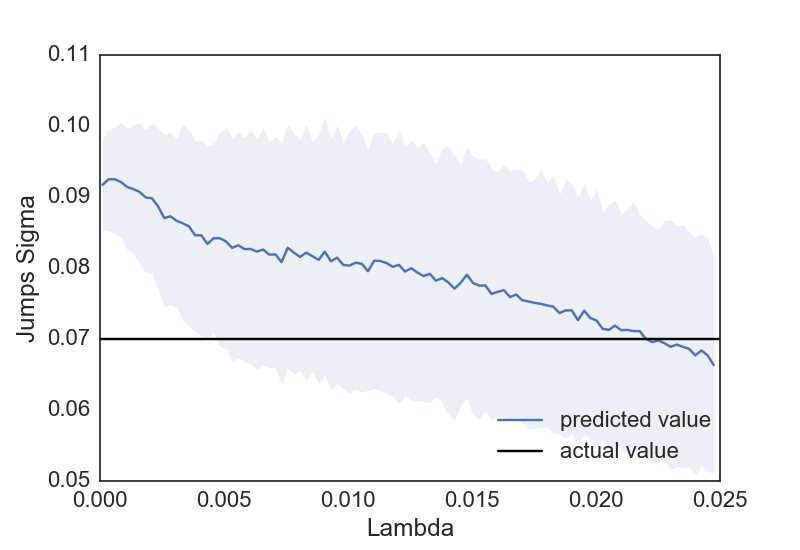
\includegraphics[width=1\linewidth]{Images/Output-Sensitivity-Results/ConvolutionalNN-MultipleOutput-ELU/Varying-Lambda/Jumps_Sigma}
			}{
				\caption{The mean $\hat{\sigma}_{jumps}$ parameter estimate plotted against the actual parameter value, $\sigma_{jumps} = 0.07$, for different values of $\lambda$.}
				\label{fig:sensitivity_test:multiple_output:varying_lambda:jumps_sigma}
			}
			
			\ffigbox{
				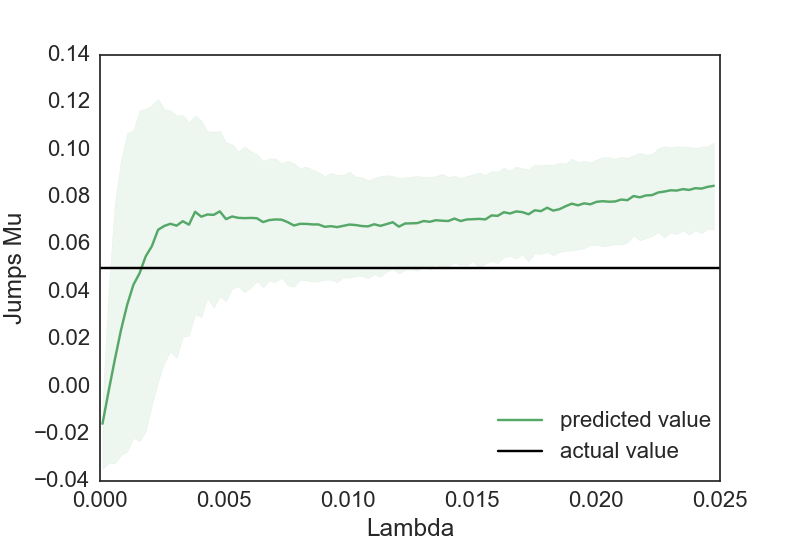
\includegraphics[width=1\linewidth]{Images/Output-Sensitivity-Results/ConvolutionalNN-MultipleOutput-ELU/Varying-Lambda/Jumps_Mu}
			}{
				\caption{The mean $\hat{\mu}_{jumps}$ parameter estimate plotted against the actual parameter value, $\mu_{jumps} = 0.05$, for different values of $\lambda$.}
				\label{fig:sensitivity_test:multiple_output:varying_lambda:jumps_mu}
			}
	\end{subfloatrow}}{
		\caption{The mean parameter estimates (with $68\%$ confidence interval) of $\hat{\mu}$, $\hat{\sigma}$, $\hat{\mu}_{jumps}$ and $\hat{\sigma}_{jumps}$, plotted against their actual values ($\mu = 0.05$, $\sigma = 0.1$, $\mu_{jumps} = 0.05$ and $\sigma_{jumps} = 0.07$), while varying the $\lambda$ parameter in the range $\left(0, 0.025\right)$.}
		\label{fig:sensitivity_test:multiple_output:varying_lambda}}
\end{figure}


\subsubsection{Variations in $\sigma_{jumps}$}

%\begin{figure}[h]
%	\centering
%	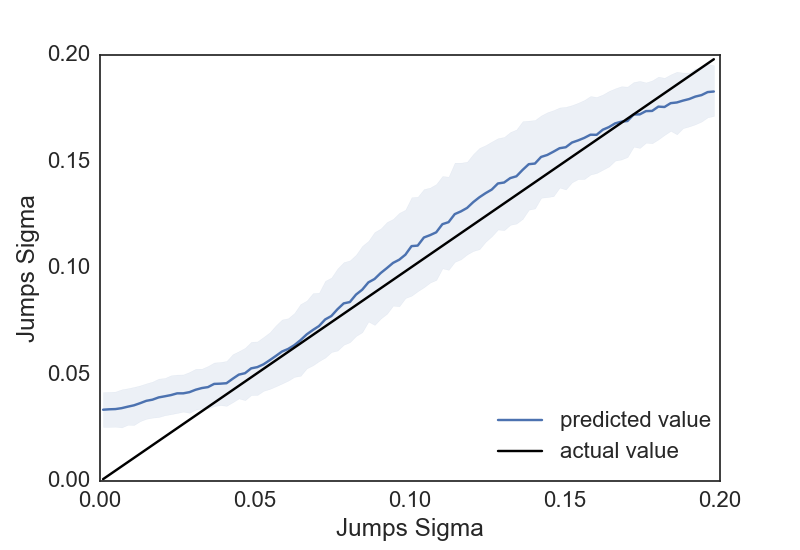
\includegraphics[width=0.7\linewidth]{Images/Output-Sensitivity-Results/ConvolutionalNN-MultipleOutput-ELU/Varying-Jumps_sigma/Jumps_Sigma}
%	\caption{The mean deviation (with $68\%$ confidence interval) of the $\hat{\sigma}_{jumps}$ parameter estimate from the actual parameter value, $\sigma_{jumps}$, for different values of $\sigma_{jumps}$. All the other parameters are kept constant as $\mu = 0.05, \sigma = 0.1, \lambda = 0.02$ and $\mu_{jumps} = 0.05$.}
%	\label{fig:sensitivity_test:multiple_output:varying_jumps_sigma:jumps_sigma}
%\end{figure}

\begin{figure}[h]
\ffigbox{
%	\begin{subfloatrow}
%		
%			\ffigbox{
%			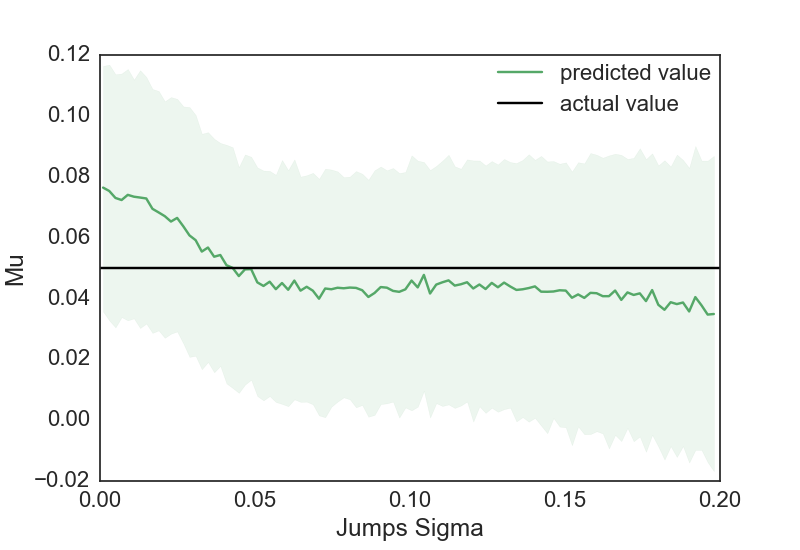
\includegraphics[width=1\linewidth]{Images/Output-Sensitivity-Results/ConvolutionalNN-MultipleOutput-ELU/Varying-Jumps_sigma/Mu}
%				}{
%			\caption{The mean $\hat{\mu}$ parameter estimate plotted against the actual parameter value, $\mu = 0.05$, for different values of $\sigma_{jumps}$.}
%				\label{fig:sensitivity_test:multiple_output:varying_jumps_sigma:mu}
%				}
%			
%			\ffigbox{	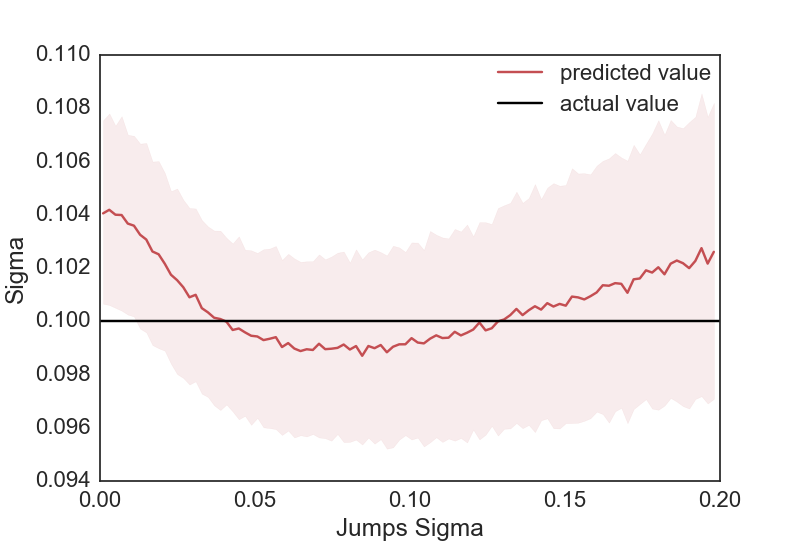
\includegraphics[width=1\linewidth]{Images/Output-Sensitivity-Results/ConvolutionalNN-MultipleOutput-ELU/Varying-Jumps_sigma/Sigma}
%			}{
%			\caption{The mean $\sigma$ parameter estimate plotted against the actual parameter value, $\sigma = 0.1$, for different values of $\sigma_{jumps}$.}
%				\label{fig:sensitivity_test:multiple_output:varying_jumps_sigma:sigma}
%				}
%			
%			\end{subfloatrow}
		\begin{subfloatrow}
		
			\ffigbox{
			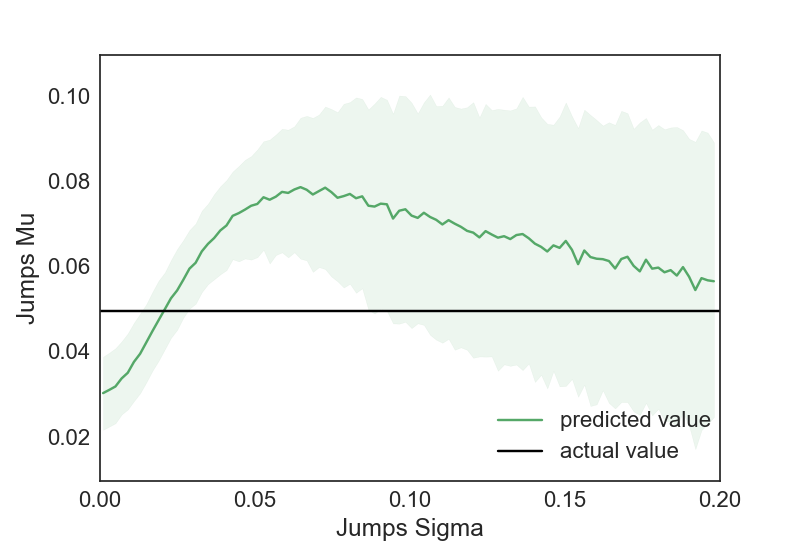
\includegraphics[width=1\linewidth]{Images/Output-Sensitivity-Results/ConvolutionalNN-MultipleOutput-ELU/Varying-Jumps_sigma/Jumps_Mu}
				}{
			\caption{The mean $\hat{\mu}_{jumps}$ parameter estimate plotted against the actual parameter value, $\mu_{jumps} = 0.05$, for different values of $\mu_{jumps}$.}
				\label{fig:sensitivity_test:multiple_output:varying_jumps_sigma:jumps_mu}
				}
			
			\ffigbox{
			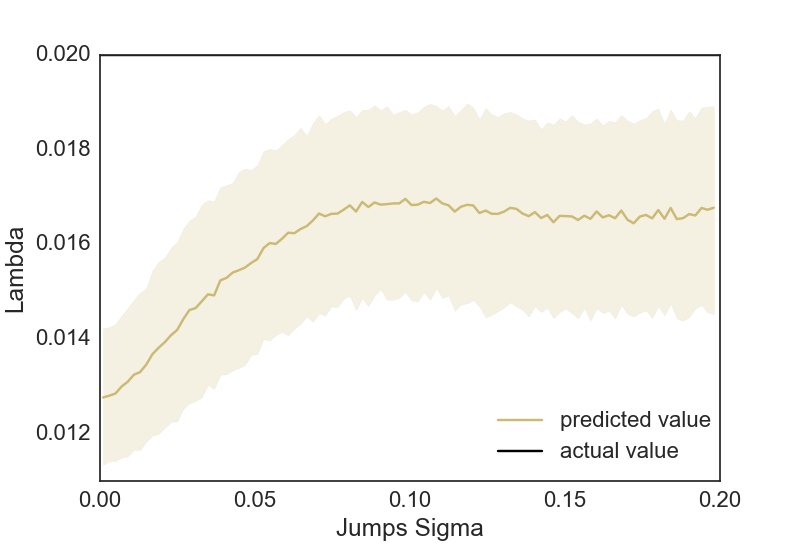
\includegraphics[width=1\linewidth]{Images/Output-Sensitivity-Results/ConvolutionalNN-MultipleOutput-ELU/Varying-Jumps_sigma/Lambda}
				}{
			\caption{The mean $\lambda$ parameter estimate plotted against the actual parameter value, $\lambda = 0.2$, for different values of $\sigma_{jumps}$.}
				\label{fig:sensitivity_test:multiple_output:varying_jumps_sigma:lambda}
				}
			\end{subfloatrow}}{
	\caption{The mean parameter estimates (with $68\%$ confidence interval) of $\hat{\mu}$, $\hat{\sigma}$, $\hat{\mu}_{jumps}$ and $\lambda$, plotted against their actual values ($\mu = 0.05$, $\sigma = 0.1$, $\mu_{jumps} = 0.05$ and $\lambda = 0.02$), while varying the $\sigma_{jumps}$ parameter in the range $\left(0, 0.2\right)$.}
		\label{fig:sensitivity_test:multiple_output:varying_jumps_sigma}}
		\end{figure}

The value of $\sigma_{jumps}$ has notable effects on the errors of the estimates of $\hat{\mu}_{jumps}$ and $\hat{\lambda}$.

As to be expected, larger $\sigma_{jumps}$ tend to lower the confidence associated with the estimate, $\hat{\mu}_{jumps}$ (Figure \ref{fig:sensitivity_test:multiple_output:varying_jumps_sigma:jumps_mu}).

Figire \ref{fig:sensitivity_test:multiple_output:varying_jumps_sigma:lambda} illustrates how $\sigma_{jumps}$ puts upward pressure on the estimate of $\lambda$. This might indicate that the model is not sure as to whether "more jumps" just means "greater volatility" in the jump sizes.

\subsubsection{Variations in $\mu_{jumps}$}

\begin{figure}[h]
	\centering
	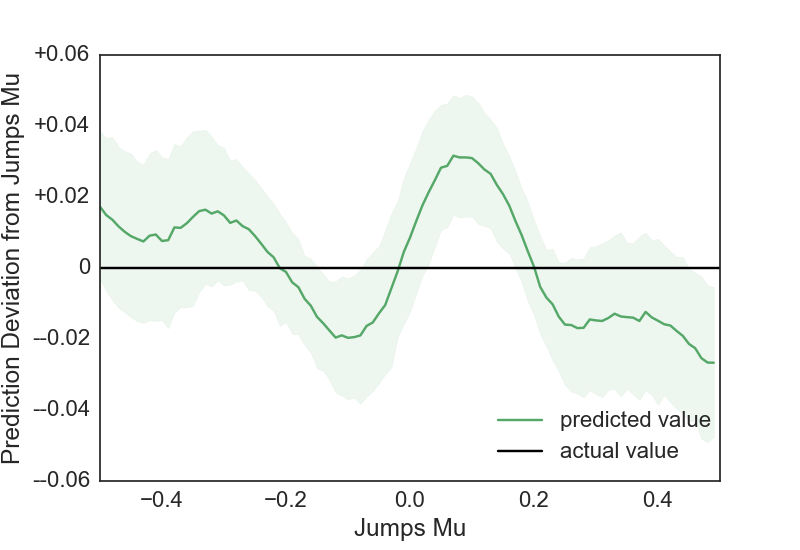
\includegraphics[width=0.5\linewidth]{Images/Output-Sensitivity-Results/ConvolutionalNN-MultipleOutput-ELU/Varying-Jumps_mu/Jumps_Mu}
	\caption{The mean deviation (with $68\%$ confidence interval) of the $\hat{\mu}_{jumps}$ parameter estimate from the actual parameter value, $\mu_{jumps}$, for different values of $\mu_{jumps}$. All the other parameters are kept constant as $\mu = 0.05, \sigma = 0.1, \lambda = 0.02$ and $\sigma_{jumps} = 0.07$.}
	\label{fig:sensitivity_test:multiple_output:varying_jumps_mu:jumps_mu}
\end{figure}

Variations in $\mu_{jumps}$ notably affect almost all of the parameter estimates produced by the \acrshort{cnn} Multiple Output model.

\begin{figure}[h]
	\ffigbox{
		\begin{subfloatrow}
			
%			\ffigbox{
%				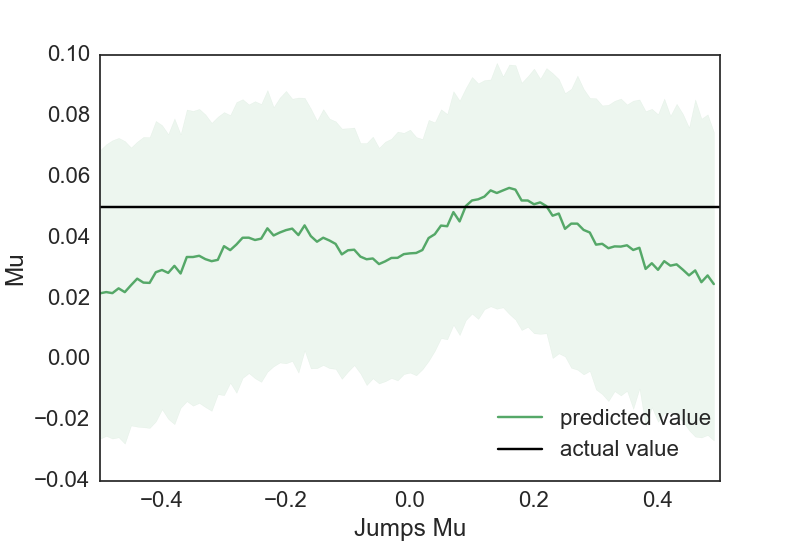
\includegraphics[width=1\linewidth]{Images/Output-Sensitivity-Results/ConvolutionalNN-MultipleOutput-ELU/Varying-Jumps_mu/Mu}
%			}{
%				\caption{The mean $\hat{\mu}$ parameter estimate plotted against the actual parameter value, $\mu = 0.05$, for different values of $\mu_{jumps}$.}
%				\label{fig:sensitivity_test:multiple_output:varying_jumps_mu:mu}
%			}
%			
			\ffigbox{	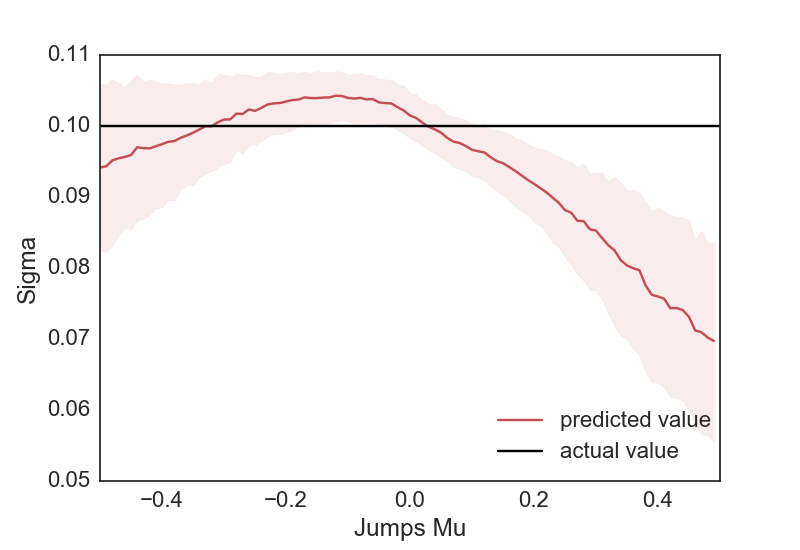
\includegraphics[width=1\linewidth]{Images/Output-Sensitivity-Results/ConvolutionalNN-MultipleOutput-ELU/Varying-Jumps_mu/Sigma}
			}{
				\caption{The mean $\sigma$ parameter estimate plotted against the actual parameter value, $\sigma = 0.1$, for different values of $\mu_{jumps}$.}
				\label{fig:sensitivity_test:multiple_output:varying_jumps_mu:sigma}
			}
%			
%		\end{subfloatrow}
%		\begin{subfloatrow}
%			
%			\ffigbox{
%				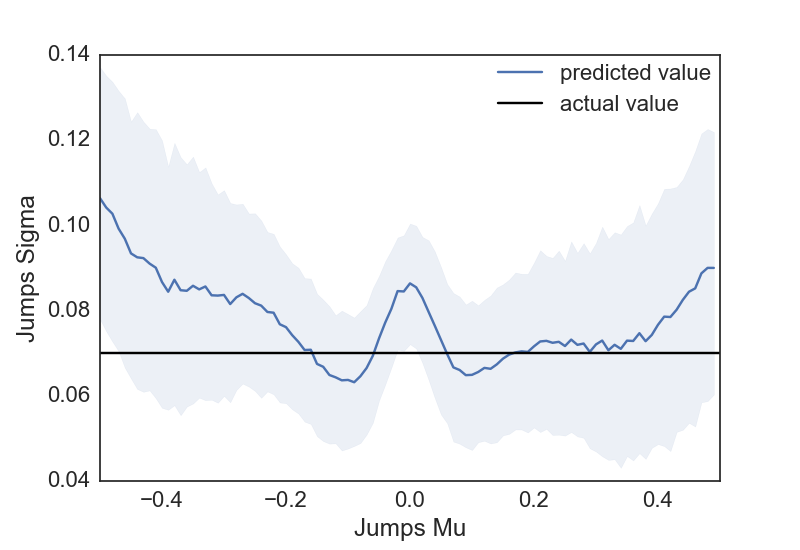
\includegraphics[width=1\linewidth]{Images/Output-Sensitivity-Results/ConvolutionalNN-MultipleOutput-ELU/Varying-Jumps_mu/Jumps_Sigma}
%			}{
%				\caption{The mean $\hat{\sigma}_{jumps}$ parameter estimate plotted against the actual parameter value, $\sigma_{jumps} = 0.07$, for different values of $\mu_{jumps}$.}
%				\label{fig:sensitivity_test:multiple_output:varying_jumps_mu:jumps_sigma}
%			}
			
			\ffigbox{
				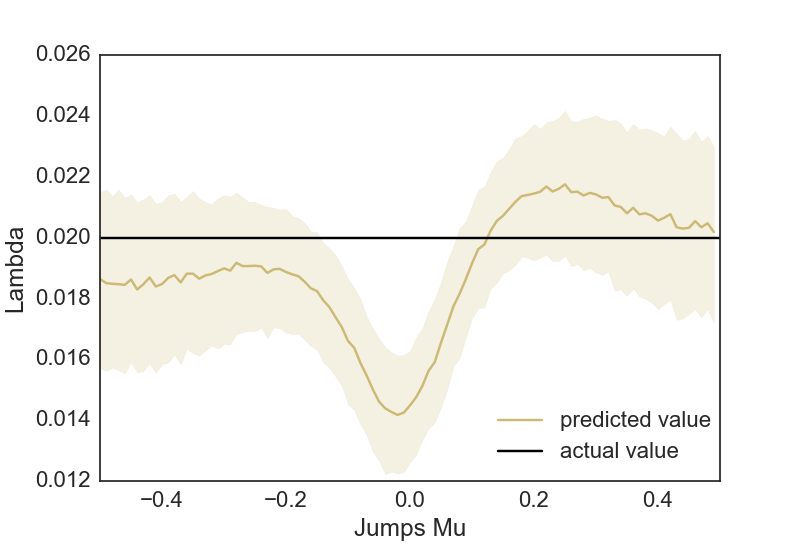
\includegraphics[width=1\linewidth]{Images/Output-Sensitivity-Results/ConvolutionalNN-MultipleOutput-ELU/Varying-Jumps_mu/Lambda}
			}{
				\caption{The mean $\lambda$ parameter estimate plotted against the actual parameter value, $\lambda = 0.2$, for different values of $\mu_{jumps}$.}
				\label{fig:sensitivity_test:multiple_output:varying_jumps_mu:lambda}
			}
	\end{subfloatrow}}{
		\caption{The mean parameter estimates (with $68\%$ confidence interval) of $\hat{\mu}$, $\hat{\sigma}$, $\hat{\sigma}_{jumps}$ and $\lambda$, plotted against their actual values ($\mu = 0.05$, $\sigma = 0.1$, $\lambda= 0.02$ and $\sigma_{jumps} = 0.07$), while varying the $\mu_{jumps}$ parameter in the range $\left(-0.5, 0.5\right)$.}
		\label{fig:sensitivity_test:multiple_output:varying_jumps_mu}}
\end{figure}

\section{Conclusion}
While a multiple output model might be more convenient to build and use, it was illustrated that single output models are quicker to train and more robust. The author's study also found that, while a fully connected architecture based on the moments and autocorrelations of the process performed well for the simpler parameters such as $\mu$ and $\sigma$, its estimates of $\lambda$ were less consistent. Figure \ref{fig:training:fully_connected_jumps} demonstrates the difficulty of training the fully connected model to estimate the $\lambda$ parameter.

In particular for the $\lambda$ parameter, a single-output convolutional model was quicker to train than either of the multiple output models (figure \ref{fig:lambda-rsquared}).

The full sets of sensitivity tests are available in Appendix \ref{appendix:sensitivity_tests}, while the results will be discussed in Chapter \ref{chapter:results}.

\chapter{Results}
\label{chapter:results}

First, the individual accuracy of the selected architectures were investigated. $1000$ simulated sample paths from a Merton Jump-Diffusion process with parameters, $\mu = 0.05$, $\sigma = 0.1$, $\lambda = 0.02$, $\mu_{jumps} = 0.05$ and $\sigma_{jumps} = 0.07$ were used. The (already trained) NN models were then used to predict these original parameters, given the set of $1000$ sample paths. 

The parameter estimation study investigated and compared results using: 
\setlist{nolistsep}
\begin{enumerate}[-]
	\itemsep0em 
	\item  \acrshort{mme},
	\item  Likelihood profiling of \citet{Honore},
	\item  \acrshort{mlestimation},
	\item a multiple output convolutional \acrshort{ann} model as defined in section \ref{chap:ConvolutionalNeuralNetwork-section:MultipleParameterPredictionArchitecture} above,
	\item a fully connected NN as defined in section \ref{subsection:fully_connected_ff_nn:architecture}, and
	\item a dedicated single output convolutional \acrshort{ann} model as defined in section \ref{chap:ConvolutionalNeuralNetwork-section:SingleParameterPredictionArchitecture} above.
\end{enumerate}
The full set of results is available in appendix \ref{appendix:results}. Selected portions thereof have been published as part of this chapter.

\subsubsection{Mu, $\mu$}
The results obtained from the CNN architecture in estimating $\mu$ compare well to that of those obtained by \acrshort{mlestimation}. Both methods exhibit bias, generally overestimating $\mu$ in the selected parameter set.
\begin{figure}[h]
	\ffigbox{
		\begin{subfloatrow}
			
			\ffigbox{\includegraphics[width=1\linewidth]{"Images/Parameter-Prediction-Results/MLE/Maximum Likelihood Estimation_Mu"}}{
				\caption[\acrshort{mlestimation}]{\acrshort{mlestimation}}
				\label{fig:results:mle-mu}}
			
			%			\ffigbox{	\includegraphics[width=1\linewidth]{"Images/Parameter-Prediction-Results/FullyConnected-MultipleOutput-ELU/Fully Connected Architecture - Multiple Output - ELU_Sigma"}}{
			%				\caption[Fully Connected Architecture - Multiple Output - EL]{Fully Connected Architecture - Multiple Output - \acrshort{elu}}
			%				\label{fig:fully-connected-architecture---multiple-output---elusigma}}
			
%			
%		\end{subfloatrow}
%		\begin{subfloatrow}
%			
			\ffigbox{\includegraphics[width=1\linewidth]{"Images/Parameter-Prediction-Results/ConvolutionalNN-MultipleOutput-ELU/Convolutional Architecture - Multiple Output - ELU_Mu"}}{
				\caption[\acrshort{cnn} Architecture - Multiple Output - \acrshort{elu}]{\acrshort{cnn} Architecture - Multiple Output - \acrshort{elu}}
				\label{fig:convolutional-architecture---multiple-output---elumu}}
			
%			\ffigbox{	\includegraphics[width=1\linewidth]{"Images/Parameter-Prediction-Results/FullyConnected-MultipleOutput-ELU/Fully Connected Architecture - Multiple Output - ELU_Mu"}}{
%				\caption[Fully Connected Architecture - Multiple Output - EL]{Fully Connected Architecture - Multiple Output - \acrshort{elu}}
%				\label{fig:fully-connected-architecture---multiple-output---elumu}}
			
		\end{subfloatrow}}{
	
	\caption{Various model distributions of the predicted values of $\mu$ with true value $0,05$. All other parameters were kept constant ($\sigma = 0.1$, $\lambda = 0.02$, $\mu_{jumps} = 0.05$ and $\sigma_{jumps} = 0.07$).}
	\label{fig:individual-parameter-estimation-results--mu}}
\end{figure}

\subsubsection{Sigma, $\sigma$}
 \acrshort{mlestimation} yields markedly accurate estimates for $\sigma$. 
\begin{figure}[h]
	\ffigbox{
		\begin{subfloatrow}
			
			\ffigbox{\includegraphics[width=1\linewidth]{"Images/Parameter-Prediction-Results/MLE/Maximum Likelihood Estimation_Sigma"}}{
				\caption[\acrshort{mlestimation}]{\acrshort{mlestimation}}
				\label{fig:results:mle-sigma}}
			
%			\ffigbox{	\includegraphics[width=1\linewidth]{"Images/Parameter-Prediction-Results/FullyConnected-MultipleOutput-ELU/Fully Connected Architecture - Multiple Output - ELU_Sigma"}}{
%				\caption[Fully Connected Architecture - Multiple Output - EL]{Fully Connected Architecture - Multiple Output - \acrshort{elu}}
%				\label{fig:fully-connected-architecture---multiple-output---elusigma}}
%			
%			
%	\end{subfloatrow}
%	\begin{subfloatrow}
%		
		\ffigbox{\includegraphics[width=1\linewidth]{"Images/Parameter-Prediction-Results/ConvolutionalNN-MultipleOutput-ELU/Convolutional Architecture - Multiple Output - ELU_Sigma"}}{
			\caption[\acrshort{cnn} Architecture - Multiple Output - \acrshort{elu}]{\acrshort{cnn} Architecture - Multiple Output - \acrshort{elu}}
			\label{fig:convolutional-architecture---multiple-output---elusigma}}
%		
%		\ffigbox{	\includegraphics[width=1\linewidth]{"Images/Parameter-Prediction-Results/FullyConnected-MultipleOutput-ELU/Fully Connected Architecture - Multiple Output - ELU_Sigma"}}{
%			\caption[Fully Connected Architecture - Multiple Output - EL]{Fully Connected Architecture - Multiple Output - \acrshort{elu}}
%			\label{fig:fully-connected-architecture---multiple-output---elusigma}}
		
		
	\end{subfloatrow}
}{
		
		\caption{Various model distributions of the predicted values of $\sigma$ with true value $0,1$.}
		\label{fig:individual-parameter-estimation-results--sigma}}
\end{figure}

\subsubsection{Lambda, $\lambda$}
In estimating $\lambda$, the single output model outshines the multiple output \acrshort{cnn}. Both provide slightly biased estimates, which could be due to the training process not having fully converged. This could be solved by training for a longer period of time on better hardware (for instance a \acrshort{gpu} with more memory).

\begin{figure}[h]
	\ffigbox{
		\begin{subfloatrow}
			
				\ffigbox{
				\includegraphics[width=1\linewidth]{"Images/Parameter-Prediction-Results/MLE/Maximum Likelihood Estimation_Lambda"}
			}{
				\caption[\acrshort{mlestimation}]{\acrshort{mlestimation}}
				\label{fig:results:mle-lambda}}
			
%			\ffigbox{\includegraphics[width=1\linewidth]{"Images/Parameter-Prediction-Results/ConvolutionalNN-MultipleOutput-ELU/Convolutional Architecture - Multiple Output - ELU_Lambda"}}{
%				\caption[\acrshort{cnn} Architecture - Multiple Output - \acrshort{elu}]{\acrshort{cnn} Architecture - Multiple Output - \acrshort{elu}}
%				\label{fig:convolutional-architecture---multiple-output---elulambda}}
%			
%			
%	\end{subfloatrow}
%	\begin{subfloatrow}
%		
%		\ffigbox{	\includegraphics[width=1\linewidth]{"Images/Parameter-Prediction-Results/FullyConnected-MultipleOutput-ELU/Fully Connected Architecture - Multiple Output - ELU_Lambda"}}{
%			\caption[Fully Connected Architecture - Multiple Output - EL]{Fully Connected Architecture - Multiple Output - \acrshort{elu}}
%			\label{fig:fully-connected-architecture---multiple-output---elulambda}}
%	
	\ffigbox{
		\includegraphics[width=1\linewidth]{"Images/Parameter-Prediction-Results/ConvolutionalNN-SingleOutput/Convolutional Architecture - Single Output - ELU_Lambda"}
	}{
		\caption[\acrshort{cnn} Architecture - Single Output - \acrshort{elu}]{\acrshort{cnn} Architecture - Single Output - \acrshort{elu}}
		\label{fig:convolutional-architecture---single-output---elulambda}}
	

	
	\end{subfloatrow}}{
		
		\caption{Various model distributions of the predicted values of $\lambda$ with true value $0,02$.}
		\label{fig:individual-parameter-estimation-results--lambda}}
\end{figure}


\subsubsection{Jumps Mu, $\mu_{jumps}$}
\acrshort{mlestimation} slightly underestimates $\mu_{jumps}$, while the \acrshort{cnn} architectures provide less certain estimates. Again, the single output model clearly outperforms the multiple output \acrshort{cnn} (see figures \ref{fig:appendix:convolutional-architecture---multiple-output---elujumps-mu} and \ref{fig:appendix:convolutional-architecture---single-output---jumps-mu} in Appendix \ref{appendix:results})

\begin{figure}[h]
	\ffigbox{
		\begin{subfloatrow}
			
			\ffigbox{
				\includegraphics[width=1\linewidth]{"Images/Parameter-Prediction-Results/MLE/Maximum Likelihood Estimation_Jumps Mu"}
			}{
				\caption[\acrshort{mlestimation}]{\acrshort{mlestimation}}
				\label{fig:results:mle-jumps_mu}}
			
%			\ffigbox{
%				\includegraphics[width=1\linewidth]{"Images/Parameter-Prediction-Results/ConvolutionalNN-MultipleOutput-ELU/Convolutional Architecture - Multiple Output - ELU_Jumps Mu"}
%			}{
%				\caption[\acrshort{cnn} Architecture - Multiple Output - \acrshort{elu}]{\acrshort{cnn} Architecture - Multiple Output - \acrshort{elu}}
%				\label{fig:convolutional-architecture---multiple-output---elujumps-mu}}
%	\end{subfloatrow}
%	\begin{subfloatrow}
%		
%		
%		\ffigbox{	\includegraphics[width=1\linewidth]{"Images/Parameter-Prediction-Results/FullyConnected-MultipleOutput-ELU/Fully Connected Architecture - Multiple Output - ELU_Jumps Mu"}
%		}{
%			\caption[Fully Connected Architecture - Multiple Output - EL]{Fully Connected Architecture - Multiple Output - \acrshort{elu}}
%			\label{fig:fully-connected-architecture---multiple-output---elujumps-mu}}
		
		\ffigbox{	\includegraphics[width=1\linewidth]{"Images/Parameter-Prediction-Results/ConvolutionalNN-SingleOutput/Convolutional Architecture - Single Output - ELU_Jumps Mu"}
	}{
	\caption[\acrshort{cnn} Architecture - Single Output - \acrshort{relu}]{\acrshort{cnn} Architecture - Single Output - \acrshort{relu}}
	\label{fig:convolutional-architecture---single-output---jumps-mu}}
	\end{subfloatrow}}{
		\caption{Various model distributions of the predicted values of $\mu_{jumps}$ with true value $0,05$.}
		\label{fig:individual-parameter-estimation-results--mu_jumps}}
\end{figure}

\subsubsection{Jumps Sigma, $\sigma_{jumps}$}
\acrshort{mlestimation} slightly underestimates $\sigma_{jumps}$, while the fully connected \acrshort{ann} architectures provide very certain - albeit biased - estimates. Both the dedicated single output and multiple output \acrshort{cnn} models provide very uncertain estimates of $\sigma_{jumps}$. This could be due to the training process not having completely converged (see figures \ref{fig:appendix:convolutional-architecture---multiple-output---elujumps-sigma} and \ref{fig:appendix:convolutional-architecture---single-output---jumps-sigma} in Appendix \ref{appendix:results}).

\begin{figure}[h]
	\ffigbox{
		\begin{subfloatrow}
			
			\ffigbox{
				\includegraphics[width=1\linewidth]{"Images/Parameter-Prediction-Results/MLE/Maximum Likelihood Estimation_Jumps Sigma"}
			}{
				\caption[\acrshort{mlestimation}]{\acrshort{mlestimation}}
				\label{fig:results:mle-jumps_sigma}}
			
%			\ffigbox{
%				\includegraphics[width=1\linewidth]{"Images/Parameter-Prediction-Results/ConvolutionalNN-MultipleOutput-ELU/Convolutional Architecture - Multiple Output - ELU_Jumps Sigma"}
%			}{
%				\caption[\acrshort{cnn} Architecture - Multiple Output - \acrshort{elu}]{\acrshort{cnn} Architecture - Multiple Output - \acrshort{elu}}
%				\label{fig:convolutional-architecture---multiple-output---elujumps-sigma}}
%			
%			
%	\end{subfloatrow}
%	\begin{subfloatrow}
%		
		\ffigbox{
			\includegraphics[width=1\linewidth]{"Images/Parameter-Prediction-Results/FullyConnected-MultipleOutput-ELU/Fully Connected Architecture - Multiple Output - ELU_Jumps Sigma"}
		}{
			\caption[Fully Connected Architecture - Multiple Output - EL]{Fully Connected Architecture - Multiple Output - \acrshort{elu}}
			\label{fig:fully-connected-architecture---multiple-output---elujumps-sigma}}
%	
%	\ffigbox{	\includegraphics[width=1\linewidth]{"Images/Parameter-Prediction-Results/ConvolutionalNN-SingleOutput/Convolutional Architecture - Single Output - ELU_Jumps Sigma"}
%	}{
%		\caption[\acrshort{cnn} Architecture - Single Output - \acrshort{relu}]{\acrshort{cnn} Architecture - Single Output - \acrshort{relu}}
%		\label{fig:convolutional-architecture---single-output---jumps-sigma}}
	\end{subfloatrow}}{
		
		\caption{Various model distributions of the predicted values of $\sigma_{jumps}$ with true value $0,07$.}
		\label{fig:individual-parameter-estimation-results--sigma_jumps}}
\end{figure}

\section{Method Comparison}

While the architectures have demonstrated the ability to yield acceptable estimates for complex stochastic processes, there are several practical considerations to take into account when using these models. This section will consider the practicality and limitations associated with using \acrshort{ann}s for calibration purposes.

\subsection{Practicality}
\acrshort{ann}s can be difficult to build and time consuming to train. Currently one needs access to a \acrfull{gpu} in order to train the models described in this paper. Even worse, the software used (Tensorflow\texttrademark \xspace \citep{tensorflow2015-whitepaper}) requires the Nvidia CUDA\textregistered \xspace parallel computing platform, which is only available on Nvidia \acrshort{gpu}s.

Even with good hardware, the training process can be time consuming. The models in this dissertation were trained using a g3 instance from \acrfull{aws} \acrfull{ec2}, which provides an Nvidia Tesla M60 \acrshort{gpu}. Despite having access to this computational power, the dedicated single output \acrshort{cnn} trained to predict $\hat{\sigma}_{jumps}$, took more than 36 hours to train.

\subsubsection{Online Versus Offline Training}
The advantage of training \acrshort{ann}s, is that the process is said to happen "offline". That means that one could train the model in advance, and only the prediction step would need to happen when actually estimating the parameters. The prediction step takes much less time than the training process. 

In contrast, the vanilla \acrshort{mlestimation} approach cannot be "trained" in advance. 

In the tests performed in this research (done on a dual-core 2,4 GHz Intel Core i5), estimating the parameters of 1000 simulations took more than 10 minutes using \acrshort{mlestimation}, almost an hour using the likelihood profiling approach of \citet{Honore}, but less than a minute using the pre-trained \acrshort{cnn}. This might differ based on the software package used and the programming language used. 

\subsection{Flexibility}
\subsubsection{Parameter Range}

The predictions of an \acrshort{ann} are solely based on the data it was trained on. This means that it would not be able to accurately predict the estimates of the parameters of any sample path it had not been exposed to in training. In this dissertation, for instance, the simulated values for $\lambda$ were kept in the range $\lambda\in [0.0001, 0.025]$. The model would thus not be able to accurately estimate $\hat{\lambda}$ for any $\lambda$ with value $\lambda > 0.025$. The traditional estimation procedures (\acrshort{mle} and \acrshort{mme}) thus offer greater flexibility in terms of the range of values they're able to accommodate.

It is also possible for \acrshort{ann} models to output nonsensical results, such as negative $\hat{\sigma}$ estimates.  

\subsubsection{Input Sequence Length}

The fully connected \acrshort{ann}s and \acrshort{cnn}s described in this paper can only accommodate an input sequence of a fixed length. That is, the sequence length is defined when the model is first built, after which all training and prediction sequences need to be of that same length. In this study, all the input sequence lengths were fixed to 2000 time steps. The  traditional procedures offer greater flexibility in terms of the sequence length that they're able to accommodate. There are workarounds to this issue, and in practice one might often decide on a specific sequence length of interest. \acrshort{rnn}s in particular are another alternative \acrshort{ann} architecture that can accommodate any input sequence length.

\chapter{Conclusion and Further Research}

This project investigated the ability of \acrshort{ann}s to estimate the parameters of a sufficiently complex \acrshort{sde}. Chapter \ref{chapter:introduction} introduced the problem of calibrating \acrshort{sde}s, and discussed the limitations of existing approaches. Chapter \ref{chapter:literature_review} presented the literature on similar studies. The concepts used throughout the dissertation were explained in Chapter \ref{chapter:methodology}, as was the methodology used in the simulation study. The simulation study itself, together with the proposed \acrshort{ann} architectures were presented in Chapter \ref{chapter:simulation_study}. Chapter \ref{chapter:results} reported on the results of the study and compared them to those obtained using traditional parameter estimation techniques such as \acrshort{mlestimation}, \acrshort{mme}, \acrshort{em} and likelihood profiling.

The simulation study demonstrated the ability of \acrshort{ann}s to act as a calibration scheme for the Merton Jump-Diffusion process. The \acrshort{cnn} architecture was able to yield acceptable parameter estimates, within realistic parameter bounds. What this means is that an \acrshort{ann} displays the ability to learn the calibration function and serve as a calibrator for a complex stochastic process. This can be done without the need to derive the likelihood function - which can be difficult to do, as demonstrated by \citet{Honore} and \citet{Mongwe}.

The models presented in this dissertation are far from optimal, with very basic properties common to most \acrshort{ann} architectures. With the advancements in neural network research, and the speed at which deep learning is currently applied to multiple unrelated fields, there is good reason to believe that neural networks have the ability to outperform traditional calibration techniques. 

\subsubsection{Further Research}
This research project aimed to demonstrate the ability of \acrshort{ann}s to act as a calibration scheme for stochastic processes. The question still remains as to whether \acrshort{ann}s could provide a \textit{universal} calibration method for the calibration of \textit{any}, arbitrarily complex stochastic process. Further research could focus on answering this question. It would be of interest to increase the accuracy of the predictions by trying different architectures, in particular: \acrshort{rnn}s (which are arguably much more appropriate for time series problems than the \acrshort{cnn} architecture used in this paper).

This paper should be extended to other, more complex stochastic processes in order to test the limits of \acrshort{ann}s as universal calibrators of stochastic processes. 

\subsubsection{Postscript}

Stochastic processes are powerful tools which can be applied to almost any time series-related problem. They offer clear, truthful representations of real-world processes in ways in which deterministic formulae cannot. Yet the underlying mathematics complicate their application. What one might hope to achieve is a democratisation of stochastic processes. Neural networks display the potential to offer actuaries the ability to implement and benefit from these statistical tools, without a background in stochastic calculus.

%\section{Practical Considerations}
%It must be noted that - at the time of writing - building and training \acrshort{ann}s is a time consuming and computationally intensive process. Overall, the author spent more than 300 GPU-hours on NVIDIA\textregistered \xspace Tesla\textregistered \xspace K80 devices implementing, training and testing the architectures presented in this dissertation. However, the progress made in the last year alone indicate that building and training \acrshort{ann}s are becoming more widely adopted, and - with that - come improvements in hardware and software tools.

\bibliographystyle{ussagus}
\bibliography{export}

\printglossary[title=Nomenclature]

\applyappendixstyling
\appendix

\chapter[Appendix A]{Merton Jump-Diffusion Process Parameters}
\label{appendix:merton_jd_parameters_effects}

\subsubsection{Mu, $\mu$}

\begin{figure}[h]
	\centering
	\includegraphics[width=0.65\linewidth]{Images/Parameter-Effects/Effects_Mu}
	\caption[The effects of changes in $\mu$ to the Merton Jump-Diffusion returns process]{The effects of changes in $\mu$ to the simulated asset price resulting from a Merton Jump-Diffusion returns process. The random seed was set constant at a value of $1234$. The other parameters are held constant at $\sigma=0.1, \lambda=0.02, \sigma_{jumps}=0.07$, and $\mu_{jumps}=0.05$.}
	\label{fig:effects_mu}
\end{figure}

\subsubsection{Sigma, $\sigma$}

\begin{figure}[h]
	\centering
	\includegraphics[width=0.65\linewidth]{Images/Parameter-Effects/Effects_Sigma}
	\caption[The effects of changes to $\sigma$ on the Merton Jump-Diffusion returns process]{The effects of changes to $\sigma$ on the simulated asset price resulting from a Merton Jump-Diffusion returns process. The random seed was set constant at a value of $1234$. The other parameters are held constant at $\mu=0.1, \lambda=0.02, \sigma_{jumps}=0.07$, and $\mu_{jumps}=0.05$.}
	\label{fig:effects_sigma}
\end{figure}

\subsubsection{Lambda, $\lambda$}

\begin{figure}[h]
	\centering
	\includegraphics[width=0.7\linewidth]{Images/Parameter-Effects/Effects_Lambda}
	\caption[The effects of changes to $\lambda$ on the Merton Jump-Diffusion returns process]{The effects of changes to $\lambda$ on the simulated asset price resulting from a Merton Jump-Diffusion returns process. The random seed was set constant at a value of $1234$. The other parameters are held constant at $\sigma=0.1, \mu=0.05, \sigma_{jumps}=0.07$, and $\mu_{jumps}=0.05$.}
	\label{fig:effects_lambda}
\end{figure}

\subsubsection{Jumps Sigma, $\sigma_{jumps}$}

\begin{figure}[h]
	\centering
	\includegraphics[width=0.7\linewidth]{Images/Parameter-Effects/Effects_Jumps_Sigma}
	\caption[The effects of changes to $\sigma_{jumps}$ on the Merton Jump-Diffusion returns process]{The effects of changes to $\sigma_{jumps}$ on the simulated asset price resulting from a Merton Jump-Diffusion returns process. The random seed was set constant at a value of $1234$. The other parameters are held constant at $\sigma=0.1, \mu=0.05, \lambda=0.03$, and $\mu_{jumps}=0.05$.}
	\label{fig:effects_jumps_sigma}
\end{figure}

\newpage
\subsubsection{Jumps Mu, $\mu_{jumps}$}

\begin{figure}[h]
	\centering
	\includegraphics[width=0.7\linewidth]{Images/Parameter-Effects/Effects_Jumps_Mu}
	\caption[The effects of changes to $\mu_{jumps}$ on the Merton Jump-Diffusion returns process]{The effects of changes to $\mu_{jumps}$ on the simulated asset price resulting from a Merton Jump-Diffusion returns process. The random seed was set constant at a value of $1234$. The other parameters are held constant at $\sigma=0.1, \mu=0.05, \lambda=0.02$, and $\sigma_{jumps}=0.07$.}
	\label{fig:effects_jumps_mu}
\end{figure}

\chapter[Appendix B]{Sensitivity Tests}
\label{appendix:sensitivity_tests}

\section{Convolutional Multiple Output Architecture}
\subsubsection{Variations in $\mu$}
\begin{figure}[!htb]
	\centering
	\includegraphics[width=0.7\linewidth]{Images/Output-Sensitivity-Results/ConvolutionalNN-MultipleOutput-ELU/Varying-Mu/Mu}
	\caption{The deviation (with $68\%$ confidence interval) of the $\hat{\mu}$ parameter estimate from the actual parameter value, $\mu$, for different values of $\mu$. All the other parameters are kept constant as $\sigma = 0.1, \lambda = 0.02, \mu_{jumps} = 0.05$ and $\sigma_{jumps} = 0.07$}
	\label{fig:appendix:sensitivity_test:multiple_output:varying_mu:mu}
\end{figure}

\begin{figure}[!htb]
	\ffigbox{
				\begin{subfloatrow}
					
					\ffigbox{
						\includegraphics[width=1\linewidth]{Images/Output-Sensitivity-Results/ConvolutionalNN-MultipleOutput-ELU/Varying-Mu/sigma}
					}{
						\caption{The $\hat{\sigma}$ parameter estimate plotted against the actual parameter value, $\sigma = 0.1$, for different values of $\mu$.}
						\label{fig:appendix:sensitivity_test:multiple_output:varying_mu:sigma}
					}
				
					\ffigbox{
					\includegraphics[width=1\linewidth]{Images/Output-Sensitivity-Results/ConvolutionalNN-MultipleOutput-ELU/Varying-Mu/Jumps_Sigma}
					}{
					\caption{The $\hat{\sigma}_{jumps}$ parameter estimate plotted against the actual parameter value, $\sigma_{jumps} = 0.07$, for different values of $\mu$.}
					\label{fig:appendix:sensitivity_test:multiple_output:varying_mu:jumps_sigma}
					}
		
				\end{subfloatrow}
		\begin{subfloatrow}
			
			\ffigbox{	\includegraphics[width=1\linewidth]{Images/Output-Sensitivity-Results/ConvolutionalNN-MultipleOutput-ELU/Varying-Mu/Lambda}
			}{
				\caption{The $\lambda$ parameter estimate plotted against the actual parameter value, $\lambda = 0.02$, for different values of $\mu$.}
				\label{fig:appendix:sensitivity_test:multiple_output:varying_mu:lambda}
			}
			
			\ffigbox{
				\includegraphics[width=1\linewidth]{Images/Output-Sensitivity-Results/ConvolutionalNN-MultipleOutput-ELU/Varying-Mu/Jumps_Mu}
			}{
				\caption{The $\hat{\mu}_{jumps}$ parameter estimate plotted against the actual parameter value, $\mu_{jumps} = 0.05$, for different values of $\mu$.}
				\label{fig:appendix:sensitivity_test:multiple_output:varying_mu:jumps_mu}
			}
	\end{subfloatrow}}{
		\caption{The parameter estimates (with $68\%$ confidence interval) of $\hat{\sigma}$, $\hat{\lambda}$, $\hat{\mu}_{jumps}$ and $\hat{\sigma}_{jumps}$, plotted against their actual values ($\sigma = 0.1$, $\lambda = 0.02$, $\mu_{jumps} = 0.05$ and $\sigma_{jumps} = 0.07$), while varying the $\mu$ parameter in the range $\left(-1.0, 1.0\right)$.}
		\label{fig:appendix:sensitivity_test:multiple_output:varying_mu}}
\end{figure}

\clearpage
\subsubsection{Variations in $\sigma$}
\begin{figure}[!htb]
	\centering
	\includegraphics[width=0.43\linewidth]{Images/Output-Sensitivity-Results/ConvolutionalNN-MultipleOutput-ELU/Varying-Sigma/Sigma}
	\caption{The deviation (with $68\%$ confidence interval) of the $\hat{\sigma}$ parameter estimate from the actual parameter value, $\sigma$, for different values of $\sigma$. All the other parameters are kept constant as $\mu = 0.05, \lambda = 0.02, \mu_{jumps} = 0.05$ and $\sigma_{jumps} = 0.07$.}
	\label{fig:appendix:sensitivity_test:multiple_output:varying_sigma:sigma}
\end{figure}

\begin{figure}[!htb]
	\ffigbox{
		\begin{subfloatrow}
			
			\ffigbox{
				\includegraphics[width=0.9\linewidth]{Images/Output-Sensitivity-Results/ConvolutionalNN-MultipleOutput-ELU/Varying-Sigma/Mu}
			}{
				\caption{The mean $\hat{\mu}$ parameter estimate plotted against the actual parameter value, $\mu = 0.05$, for different values of $\sigma$.}
				\label{fig:appendix:sensitivity_test:multiple_output:varying_sigma:mu}
			}
			
			\ffigbox{	\includegraphics[width=0.9\linewidth]{Images/Output-Sensitivity-Results/ConvolutionalNN-MultipleOutput-ELU/Varying-Sigma/Lambda}
			}{
				\caption{The mean $\lambda$ parameter estimate plotted against the actual parameter value, $\lambda = 0.02$, for different values of $\sigma$.}
				\label{fig:appendix:sensitivity_test:multiple_output:varying_sigma:lambda}
			}
			
		\end{subfloatrow}
				\begin{subfloatrow}
					
					\ffigbox{
						\includegraphics[width=0.9\linewidth]{Images/Output-Sensitivity-Results/ConvolutionalNN-MultipleOutput-ELU/Varying-Sigma/Jumps_Sigma}
					}{
						\caption{The mean $\hat{\sigma}_{jumps}$ parameter estimate plotted against the actual parameter value, $\sigma_{jumps} = 0.07$, for different values of $\sigma$.}
						\label{fig:appendix:sensitivity_test:multiple_output:varying_sigma:jumps_sigma}
					}
					
					\ffigbox{
						\includegraphics[width=0.9\linewidth]{Images/Output-Sensitivity-Results/ConvolutionalNN-MultipleOutput-ELU/Varying-Sigma/Jumps_Mu}
					}{
						\caption{The mean $\hat{\mu}_{jumps}$ parameter estimate plotted against the actual parameter value, $\mu_{jumps} = 0.05$, for different values of $\sigma$.}
						\label{fig:appendix:sensitivity_test:multiple_output:varying_sigma:jumps_mu}
					}
			\end{subfloatrow}
	}{
		\caption{The mean parameter estimates (with $68\%$ confidence interval) of $\hat{\mu}$, $\hat{\lambda}$, $\hat{\mu}_{jumps}$ and $\hat{\sigma}_{jumps}$, plotted against their actual values ($\mu = 0.05$, $\lambda = 0.02$, $\mu_{jumps} = 0.05$ and $\sigma_{jumps} = 0.07$), while varying the $\sigma$ parameter in the range $\left(0, 0.2\right)$.}
		\label{fig:appendix:sensitivity_test:multiple_output:varying_sigma}}
\end{figure}

\clearpage
\subsubsection{Variations in $\lambda$}
\begin{figure}[h]
	\centering
	\includegraphics[width=0.43\linewidth]{Images/Output-Sensitivity-Results/ConvolutionalNN-MultipleOutput-ELU/Varying-Lambda/Lambda}
	\caption{The mean deviation (with $68\%$ confidence interval) of the $\hat{\lambda}$ parameter estimate from the actual parameter value, $\lambda$, for different values of $\lambda$. All the other parameters are kept constant as $\mu = 0.05, \sigma = 0.1, \mu_{jumps} = 0.05$ and $\sigma_{jumps} = 0.07$.}
	\label{fig:appendix:sensitivity_test:multiple_output:varying_lambda:lambda}
\end{figure}

\begin{figure}[h]
	\ffigbox{
				\begin{subfloatrow}
					
					\ffigbox{
						\includegraphics[width=0.9\linewidth]{Images/Output-Sensitivity-Results/ConvolutionalNN-MultipleOutput-ELU/Varying-Lambda/Mu}
					}{
						\caption{The mean $\hat{\mu}$ parameter estimate plotted against the actual parameter value, $\mu = 0.05$, for different values of $\lambda$.}
						\label{fig:appendix:sensitivity_test:multiple_output:varying_lambda:mu}
					}
					
					\ffigbox{	\includegraphics[width=0.9\linewidth]{Images/Output-Sensitivity-Results/ConvolutionalNN-MultipleOutput-ELU/Varying-Lambda/Sigma}
					}{
						\caption{The mean $\sigma$ parameter estimate plotted against the actual parameter value, $\sigma = 0.1$, for different values of $\lambda$.}
						\label{fig:appendix:sensitivity_test:multiple_output:varying_lambda:sigma}
					}
					
				\end{subfloatrow}
		\begin{subfloatrow}
			
			\ffigbox{
				\includegraphics[width=0.9\linewidth]{Images/Output-Sensitivity-Results/ConvolutionalNN-MultipleOutput-ELU/Varying-Lambda/Jumps_Sigma}
			}{
				\caption{The mean $\hat{\sigma}_{jumps}$ parameter estimate plotted against the actual parameter value, $\sigma_{jumps} = 0.07$, for different values of $\lambda$.}
				\label{fig:appendix:sensitivity_test:multiple_output:varying_lambda:jumps_sigma}
			}
			
			\ffigbox{
				\includegraphics[width=0.9\linewidth]{Images/Output-Sensitivity-Results/ConvolutionalNN-MultipleOutput-ELU/Varying-Lambda/Jumps_Mu}
			}{
				\caption{The mean $\hat{\mu}_{jumps}$ parameter estimate plotted against the actual parameter value, $\mu_{jumps} = 0.05$, for different values of $\lambda$.}
				\label{fig:appendix:sensitivity_test:multiple_output:varying_lambda:jumps_mu}
			}
	\end{subfloatrow}}{
		\caption{The mean parameter estimates (with $68\%$ confidence interval) of $\hat{\mu}$, $\hat{\sigma}$, $\hat{\mu}_{jumps}$ and $\hat{\sigma}_{jumps}$, plotted against their actual values ($\mu = 0.05$, $\sigma = 0.1$, $\mu_{jumps} = 0.05$ and $\sigma_{jumps} = 0.07$), while varying the $\lambda$ parameter in the range $\left(0, 0.025\right)$.}
		\label{fig:appendix:sensitivity_test:multiple_output:varying_lambda}}
\end{figure}

\clearpage
\subsubsection{Variations in $\sigma_{jumps}$}
\begin{figure}[h]
	\centering
	\includegraphics[width=0.43\linewidth]{Images/Output-Sensitivity-Results/ConvolutionalNN-MultipleOutput-ELU/Varying-Jumps_sigma/Jumps_Sigma}
	\caption{The mean deviation (with $68\%$ confidence interval) of the $\hat{\sigma}_{jumps}$ parameter estimate from the actual parameter value, $\sigma_{jumps}$, for different values of $\sigma_{jumps}$. All the other parameters are kept constant as $\mu = 0.05, \sigma = 0.1, \lambda = 0.02$ and $\mu_{jumps} = 0.05$.}
	\label{fig:appendix:sensitivity_test:multiple_output:varying_jumps_sigma:jumps_sigma}
\end{figure}

\begin{figure}[h]
	\ffigbox{
			\begin{subfloatrow}
				
					\ffigbox{
					\includegraphics[width=0.9\linewidth]{Images/Output-Sensitivity-Results/ConvolutionalNN-MultipleOutput-ELU/Varying-Jumps_sigma/Mu}
						}{
					\caption{The mean $\hat{\mu}$ parameter estimate plotted against the actual parameter value, $\mu = 0.05$, for different values of $\sigma_{jumps}$.}
						\label{fig:appendix:sensitivity_test:multiple_output:varying_jumps_sigma:mu}
						}
					
					\ffigbox{	\includegraphics[width=0.9\linewidth]{Images/Output-Sensitivity-Results/ConvolutionalNN-MultipleOutput-ELU/Varying-Jumps_sigma/Sigma}
					}{
					\caption{The mean $\sigma$ parameter estimate plotted against the actual parameter value, $\sigma = 0.1$, for different values of $\sigma_{jumps}$.}
						\label{fig:appendix:sensitivity_test:multiple_output:varying_jumps_sigma:sigma}
						}
					
					\end{subfloatrow}
		\begin{subfloatrow}
			
			\ffigbox{
				\includegraphics[width=0.9\linewidth]{Images/Output-Sensitivity-Results/ConvolutionalNN-MultipleOutput-ELU/Varying-Jumps_sigma/Jumps_Mu}
			}{
				\caption{The mean $\hat{\mu}_{jumps}$ parameter estimate plotted against the actual parameter value, $\mu_{jumps} = 0.05$, for different values of $\mu_{jumps}$.}
				\label{fig:appendix:sensitivity_test:multiple_output:varying_jumps_sigma:jumps_mu}
			}
			
			\ffigbox{
				\includegraphics[width=0.9\linewidth]{Images/Output-Sensitivity-Results/ConvolutionalNN-MultipleOutput-ELU/Varying-Jumps_sigma/Lambda}
			}{
				\caption{The mean $\lambda$ parameter estimate plotted against the actual parameter value, $\lambda = 0.2$, for different values of $\sigma_{jumps}$.}
				\label{fig:appendix:sensitivity_test:multiple_output:varying_jumps_sigma:lambda}
			}
	\end{subfloatrow}}{
		\caption{The mean parameter estimates (with $68\%$ confidence interval) of $\hat{\mu}$, $\hat{\sigma}$, $\hat{\mu}_{jumps}$ and $\lambda$, plotted against their actual values ($\mu = 0.05$, $\sigma = 0.1$, $\mu_{jumps} = 0.05$ and $\lambda = 0.02$), while varying the $\sigma_{jumps}$ parameter in the range $\left(0, 0.2\right)$.}
		\label{fig:appendix:sensitivity_test:multiple_output:varying_jumps_sigma}}
\end{figure}

\clearpage
\subsubsection{Variations in $\mu_{jumps}$}
\begin{figure}[h]
	\centering
	\includegraphics[width=0.43\linewidth]{Images/Output-Sensitivity-Results/ConvolutionalNN-MultipleOutput-ELU/Varying-Jumps_mu/Jumps_Mu}
	\caption{The mean deviation (with $68\%$ confidence interval) of the $\hat{\mu}_{jumps}$ parameter estimate from the actual parameter value, $\mu_{jumps}$, for different values of $\mu_{jumps}$. All the other parameters are kept constant as $\mu = 0.05, \sigma = 0.1, \lambda = 0.02$ and $\sigma_{jumps} = 0.07$.}
	\label{fig:appendix:sensitivity_test:multiple_output:varying_jumps_mu:jumps_mu}
\end{figure}

\begin{figure}[h]
	\ffigbox{
		\begin{subfloatrow}
			
			\ffigbox{
				\includegraphics[width=0.9\linewidth]{Images/Output-Sensitivity-Results/ConvolutionalNN-MultipleOutput-ELU/Varying-Jumps_mu/Mu}
			}{
				\caption{The mean $\hat{\mu}$ parameter estimate plotted against the actual parameter value, $\mu = 0.05$, for different values of $\mu_{jumps}$.}
				\label{fig:appendix:sensitivity_test:multiple_output:varying_jumps_mu:mu}
			}
			
			\ffigbox{	\includegraphics[width=0.9\linewidth]{Images/Output-Sensitivity-Results/ConvolutionalNN-MultipleOutput-ELU/Varying-Jumps_mu/Sigma}
			}{
				\caption{The mean $\sigma$ parameter estimate plotted against the actual parameter value, $\sigma = 0.1$, for different values of $\mu_{jumps}$.}
				\label{fig:appendix:sensitivity_test:multiple_output:varying_jumps_mu:sigma}
			}
			
		\end{subfloatrow}
		\begin{subfloatrow}
			
			\ffigbox{
				\includegraphics[width=0.9\linewidth]{Images/Output-Sensitivity-Results/ConvolutionalNN-MultipleOutput-ELU/Varying-Jumps_mu/Jumps_Sigma}
			}{
				\caption{The mean $\hat{\sigma}_{jumps}$ parameter estimate plotted against the actual parameter value, $\sigma_{jumps} = 0.07$, for different values of $\mu_{jumps}$.}
				\label{fig:appendix:sensitivity_test:multiple_output:varying_jumps_mu:jumps_sigma}
			}
			
			\ffigbox{
				\includegraphics[width=0.9\linewidth]{Images/Output-Sensitivity-Results/ConvolutionalNN-MultipleOutput-ELU/Varying-Jumps_mu/Lambda}
			}{
				\caption{The mean $\lambda$ parameter estimate plotted against the actual parameter value, $\lambda = 0.2$, for different values of $\mu_{jumps}$.}
				\label{fig:appendix:sensitivity_test:multiple_output:varying_jumps_mu:lambda}
			}
	\end{subfloatrow}}{
		\caption{The mean parameter estimates (with $68\%$ confidence interval) of $\hat{\mu}$, $\hat{\sigma}$, $\hat{\sigma}_{jumps}$ and $\lambda$, plotted against their actual values ($\mu = 0.05$, $\sigma = 0.1$, $\lambda= 0.02$ and $\sigma_{jumps} = 0.07$), while varying the $\mu_{jumps}$ parameter in the range $\left(-0.5, 0.5\right)$.}
		\label{fig:appendix:sensitivity_test:multiple_output:varying_jumps_mu}}
\end{figure}

%\clearpage
%\section{Convolutional Single Output Architecture}

\chapter[Appendix C]{Results}
\label{appendix:results}

This chapter documents the individual accuracy of the investigated architectures, comparing each with the results obtained using more traditional methods such as \acrshort{mlestimation}, \acrshort{mme} and the likelihood profiling method of \citet{Honore}. $1000$ simulated sample paths from a Merton Jump-Diffusion process with parameters, $\mu = 0.05$, $\sigma = 0.1$, $\lambda = 0.02$, $\mu_{jumps} = 0.05$ and $\sigma_{jumps} = 0.07$ were used. The (already trained) NN models were then used to predict these original parameters, given the set of $1000$ sample paths. Figures \ref{fig:appendix:individual-parameter-estimation-results--mu}, \ref{fig:appendix:individual-parameter-estimation-results--sigma}, \ref{fig:appendix:individual-parameter-estimation-results--lambda}, \ref{fig:appendix:individual-parameter-estimation-results--mu_jumps}, and \ref{fig:appendix:individual-parameter-estimation-results--sigma_jumps} illustrate the parameter estimation results for $\mu, \sigma, \lambda, \mu_{jumps}$ and $\sigma_{jumps}$ using: 

\setlist{nolistsep}
\begin{enumerate}[a)]
	\itemsep0em 
	\item  \acrshort{mme}
	\item  Likelihood profiling of \citet{Honore}
	\item  \acrshort{mlestimation},
	\item a multiple output convolutional \acrshort{ann} model as defined in section \ref{chap:ConvolutionalNeuralNetwork-section:MultipleParameterPredictionArchitecture} above,
	\item a fully connected NN as defined in section \ref{subsection:fully_connected_ff_nn:architecture}, and
	\item a dedicated single output convolutional \acrshort{ann} model as defined in section \ref{chap:ConvolutionalNeuralNetwork-section:SingleParameterPredictionArchitecture} above.

\end{enumerate}

All the parameter estimates produced by \acrshort{mlestimation}, \acrshort{mme} and the likelihood profiling approach of \citet{Honore} were obtained using the R-code provided by \citet{Mongwe}.

\begin{figure}[h]
	\ffigbox{
		
		\begin{subfloatrow}
			
			\ffigbox{\includegraphics[width=1\linewidth]{"Images/Parameter-Prediction-Results/MME/Generalised Method of Moments Estimation_Mu"}}{
				\caption[\acrshort{mme}]{\acrshort{mme}}
				\label{fig:appendix:mme-mu}}
			
			\ffigbox{\includegraphics[width=1\linewidth]{"Images/Parameter-Prediction-Results/Profiling/Likelihood Profiling (Honore)_Mu"}}{
			\caption[Likelihood Profiling \citep{Honore}]{Likelihood Profiling \citep{Honore}}
			\label{fig:appendix:profiling-mu}}
	
		\end{subfloatrow}
		\begin{subfloatrow}
			
			\ffigbox{\includegraphics[width=1\linewidth]{"Images/Parameter-Prediction-Results/MLE/Maximum Likelihood Estimation_Mu"}}{
				\caption[\acrshort{mlestimation}]{\acrshort{mlestimation}}
				\label{fig:appendix:mle-mu}}
			
			%			\ffigbox{	\includegraphics[width=1\linewidth]{"Images/Parameter-Prediction-Results/FullyConnected-MultipleOutput-ELU/Fully Connected Architecture - Multiple Output - ELU_Sigma"}}{
			%				\caption[Fully Connected Architecture - Multiple Output - EL]{Fully Connected Architecture - Multiple Output - \acrshort{elu}}
			%				\label{fig:fully-connected-architecture---multiple-output---elusigma}}
			
			
		\end{subfloatrow}
		\begin{subfloatrow}
			
			\ffigbox{\includegraphics[width=1\linewidth]{"Images/Parameter-Prediction-Results/ConvolutionalNN-MultipleOutput-ELU/Convolutional Architecture - Multiple Output - ELU_Mu"}}{
				\caption[\acrshort{cnn} Architecture - Multiple Output - \acrshort{elu}]{\acrshort{cnn} Architecture - Multiple Output - \acrshort{elu}}
				\label{fig:appendix:convolutional-architecture---multiple-output---elumu}}
			
			\ffigbox{	\includegraphics[width=1\linewidth]{"Images/Parameter-Prediction-Results/FullyConnected-MultipleOutput-ELU/Fully Connected Architecture - Multiple Output - ELU_Mu"}}{
				\caption[Fully Connected Architecture - Multiple Output - EL]{Fully Connected Architecture - Multiple Output - \acrshort{elu}}
				\label{fig:appendix:fully-connected-architecture---multiple-output---elumu}}
			
	\end{subfloatrow}}{
		
		\caption{Various model distributions of the predicted values of $\mu$ with true value $0,05$.}
		\label{fig:appendix:individual-parameter-estimation-results--mu}}
\end{figure}

\begin{figure}[h]
	\ffigbox{
		
		\begin{subfloatrow}
			
			\ffigbox{\includegraphics[width=1\linewidth]{"Images/Parameter-Prediction-Results/MME/Generalised Method of Moments Estimation_Sigma"}}{
				\caption[\acrshort{mme}]{\acrshort{mme}}
				\label{fig:appendix:mme-sigma}}
			
			\ffigbox{\includegraphics[width=1\linewidth]{"Images/Parameter-Prediction-Results/Profiling/Likelihood Profiling (Honore)_Sigma"}}{
				\caption[Likelihood Profiling \citep{Honore}]{Likelihood Profiling \citep{Honore}}
				\label{fig:appendix:profiling-sigma}}
			
		\end{subfloatrow}
		\begin{subfloatrow}
			
			\ffigbox{\includegraphics[width=1\linewidth]{"Images/Parameter-Prediction-Results/MLE/Maximum Likelihood Estimation_Sigma"}}{
				\caption[\acrshort{mlestimation}]{\acrshort{mlestimation}}
				\label{fig:appendix:mle-sigma}}
			
			%			\ffigbox{	\includegraphics[width=1\linewidth]{"Images/Parameter-Prediction-Results/FullyConnected-MultipleOutput-ELU/Fully Connected Architecture - Multiple Output - ELU_Sigma"}}{
			%				\caption[Fully Connected Architecture - Multiple Output - EL]{Fully Connected Architecture - Multiple Output - \acrshort{elu}}
			%				\label{fig:fully-connected-architecture---multiple-output---elusigma}}
			
			
		\end{subfloatrow}
		\begin{subfloatrow}
			
			\ffigbox{\includegraphics[width=1\linewidth]{"Images/Parameter-Prediction-Results/ConvolutionalNN-MultipleOutput-ELU/Convolutional Architecture - Multiple Output - ELU_Sigma"}}{
				\caption[\acrshort{cnn} Architecture - Multiple Output - \acrshort{elu}]{\acrshort{cnn} Architecture - Multiple Output - \acrshort{elu}}
				\label{fig:appendix:convolutional-architecture---multiple-output---elusigma}}
			
			\ffigbox{	\includegraphics[width=1\linewidth]{"Images/Parameter-Prediction-Results/FullyConnected-MultipleOutput-ELU/Fully Connected Architecture - Multiple Output - ELU_Sigma"}}{
				\caption[Fully Connected Architecture - Multiple Output - EL]{Fully Connected Architecture - Multiple Output - \acrshort{elu}}
				\label{fig:appendix:fully-connected-architecture---multiple-output---elusigma}}
			
			
		\end{subfloatrow}
	}{
		
		\caption{Various model distributions of the predicted values of $\sigma$ with true value $0,1$.}
		\label{fig:appendix:individual-parameter-estimation-results--sigma}}
\end{figure}

\begin{figure}[h]
	\ffigbox{
		
		\begin{subfloatrow}
			
			\ffigbox{\includegraphics[width=1\linewidth]{"Images/Parameter-Prediction-Results/MME/Generalised Method of Moments Estimation_Lambda"}}{
				\caption[\acrshort{mme}]{\acrshort{mme}}
				\label{fig:appendix:mme-lambda}}
			
			\ffigbox{\includegraphics[width=1\linewidth]{"Images/Parameter-Prediction-Results/Profiling/Likelihood Profiling (Honore)_Lambda"}}{
				\caption[Likelihood Profiling \citep{Honore}]{Likelihood Profiling \citep{Honore}}
				\label{fig:appendix:profiling-lambda}}
			
		\end{subfloatrow}
		\begin{subfloatrow}
			
			\ffigbox{
				\includegraphics[width=1\linewidth]{"Images/Parameter-Prediction-Results/MLE/Maximum Likelihood Estimation_Lambda"}
			}{
				\caption[\acrshort{mlestimation}]{\acrshort{mlestimation}}
				\label{fig:appendix:mle-lambda}}
			
			\ffigbox{\includegraphics[width=1\linewidth]{"Images/Parameter-Prediction-Results/ConvolutionalNN-MultipleOutput-ELU/Convolutional Architecture - Multiple Output - ELU_Lambda"}}{
				\caption[\acrshort{cnn} Architecture - Multiple Output - \acrshort{elu}]{\acrshort{cnn} Architecture - Multiple Output - \acrshort{elu}}
				\label{fig:appendix:convolutional-architecture---multiple-output---elulambda}}
			
			
		\end{subfloatrow}
		\begin{subfloatrow}
			
			\ffigbox{	\includegraphics[width=1\linewidth]{"Images/Parameter-Prediction-Results/FullyConnected-MultipleOutput-ELU/Fully Connected Architecture - Multiple Output - ELU_Lambda"}}{
				\caption[Fully Connected Architecture - Multiple Output - EL]{Fully Connected Architecture - Multiple Output - \acrshort{elu}}
				\label{fig:appendix:fully-connected-architecture---multiple-output---elulambda}}
			
			\ffigbox{
				\includegraphics[width=1\linewidth]{"Images/Parameter-Prediction-Results/ConvolutionalNN-SingleOutput/Convolutional Architecture - Single Output - ELU_Lambda"}
			}{
				\caption[\acrshort{cnn} Architecture - Single Output - \acrshort{elu}]{\acrshort{cnn} Architecture - Single Output - \acrshort{elu}}
				\label{fig:appendix:convolutional-architecture---single-output---elulambda}}
			
			
			
	\end{subfloatrow}}{
		
		\caption{Various model distributions of the predicted values of $\lambda$ with true value $0,02$.}
		\label{fig:appendix:individual-parameter-estimation-results--lambda}}
\end{figure}

\begin{figure}[h]
	\ffigbox{
		
		\begin{subfloatrow}
			
			\ffigbox{\includegraphics[width=1\linewidth]{"Images/Parameter-Prediction-Results/MME/Generalised Method of Moments Estimation_Jumps Mu"}}{
				\caption[\acrshort{mme}]{\acrshort{mme}}
				\label{fig:appendix:mme-jumps_mu}}
			
			\ffigbox{\includegraphics[width=1\linewidth]{"Images/Parameter-Prediction-Results/Profiling/Likelihood Profiling (Honore)_Jumps Mu"}}{
				\caption[Likelihood Profiling \citep{Honore}]{Likelihood Profiling \citep{Honore}}
				\label{fig:appendix:profiling-jumps_mu}}
			
		\end{subfloatrow}
		\begin{subfloatrow}
			
			\ffigbox{
				\includegraphics[width=1\linewidth]{"Images/Parameter-Prediction-Results/MLE/Maximum Likelihood Estimation_Jumps Mu"}
			}{
				\caption[\acrshort{mlestimation}]{\acrshort{mlestimation}}
				\label{fig:appendix:mle_jumps_mu}}
			
			\ffigbox{
				\includegraphics[width=1\linewidth]{"Images/Parameter-Prediction-Results/ConvolutionalNN-MultipleOutput-ELU/Convolutional Architecture - Multiple Output - ELU_Jumps Mu"}
			}{
				\caption[\acrshort{cnn} Architecture - Multiple Output - \acrshort{elu}]{\acrshort{cnn} Architecture - Multiple Output - \acrshort{elu}}
				\label{fig:appendix:convolutional-architecture---multiple-output---elujumps-mu}}
		\end{subfloatrow}
		\begin{subfloatrow}
			
			
			\ffigbox{	\includegraphics[width=1\linewidth]{"Images/Parameter-Prediction-Results/FullyConnected-MultipleOutput-ELU/Fully Connected Architecture - Multiple Output - ELU_Jumps Mu"}
			}{
				\caption[Fully Connected Architecture - Multiple Output - EL]{Fully Connected Architecture - Multiple Output - \acrshort{elu}}
				\label{fig:appendix:fully-connected-architecture---multiple-output---elujumps-mu}}
			
			\ffigbox{	\includegraphics[width=1\linewidth]{"Images/Parameter-Prediction-Results/ConvolutionalNN-SingleOutput/Convolutional Architecture - Single Output - ELU_Jumps Mu"}
			}{
				\caption[\acrshort{cnn} Architecture - Single Output - \acrshort{relu}]{\acrshort{cnn} Architecture - Single Output - \acrshort{relu}}
				\label{fig:appendix:convolutional-architecture---single-output---jumps-mu}}
	\end{subfloatrow}}{
		\caption{Various model distributions of the predicted values of $\mu_{jumps}$ with true value $0,05$.}
		\label{fig:appendix:individual-parameter-estimation-results--mu_jumps}}
\end{figure}

\begin{figure}[h]
	\ffigbox{
		
		\begin{subfloatrow}
			
			\ffigbox{\includegraphics[width=1\linewidth]{"Images/Parameter-Prediction-Results/MME/Generalised Method of Moments Estimation_Jumps Sigma"}}{
				\caption[\acrshort{mme}]{\acrshort{mme}}
				\label{fig:appendix:mme-Jumps_Sigma}}
			
			\ffigbox{\includegraphics[width=1\linewidth]{"Images/Parameter-Prediction-Results/Profiling/Likelihood Profiling (Honore)_Jumps Sigma"}}{
				\caption[Likelihood Profiling \citep{Honore}]{Likelihood Profiling \citep{Honore}}
				\label{fig:appendix:profiling-Jumps_Sigma}}
			
		\end{subfloatrow}
		\begin{subfloatrow}
			
			\ffigbox{
				\includegraphics[width=1\linewidth]{"Images/Parameter-Prediction-Results/MLE/Maximum Likelihood Estimation_Jumps Sigma"}
			}{
				\caption[\acrshort{mlestimation}]{\acrshort{mlestimation}}
				\label{fig:appendix:mle_Jumps_Sigma}}
			
			\ffigbox{
				\includegraphics[width=1\linewidth]{"Images/Parameter-Prediction-Results/ConvolutionalNN-MultipleOutput-ELU/Convolutional Architecture - Multiple Output - ELU_Jumps Sigma"}
			}{
				\caption[\acrshort{cnn} Architecture - Multiple Output - \acrshort{elu}]{\acrshort{cnn} Architecture - Multiple Output - \acrshort{elu}}
				\label{fig:appendix:convolutional-architecture---multiple-output---elujumps-sigma}}
			
			
		\end{subfloatrow}
		\begin{subfloatrow}
			
			\ffigbox{
				\includegraphics[width=1\linewidth]{"Images/Parameter-Prediction-Results/FullyConnected-MultipleOutput-ELU/Fully Connected Architecture - Multiple Output - ELU_Jumps Sigma"}
			}{
				\caption[Fully Connected Architecture - Multiple Output - EL]{Fully Connected Architecture - Multiple Output - \acrshort{elu}}
				\label{fig:appendix:fully-connected-architecture---multiple-output---elujumps-sigma}}
			
			\ffigbox{	\includegraphics[width=1\linewidth]{"Images/Parameter-Prediction-Results/ConvolutionalNN-SingleOutput/Convolutional Architecture - Single Output - ELU_Jumps Sigma"}
			}{
				\caption[\acrshort{cnn} Architecture - Single Output - \acrshort{relu}]{\acrshort{cnn} Architecture - Single Output - \acrshort{relu}}
				\label{fig:appendix:convolutional-architecture---single-output---jumps-sigma}}
	\end{subfloatrow}}{
		
		\caption{Various model distributions of the predicted values of $\sigma_{jumps}$ with true value $0,07$.}
		\label{fig:appendix:individual-parameter-estimation-results--sigma_jumps}}
\end{figure}

\chapter[Appendix D]{List of Software Used}
\label{list_of_software_used}
\def\arraystretch{2}
\begin{tabular}[h]{l p{9cm} ll}
	
	\textbf{IPython} & A command shell for interactive computing. &\cite{ipython} \\ 
	
	\textbf{Keras} & A high-level neural networks API, written in Python running on top of TensorFlow. &\cite{chollet2015keras} \\ 
	
	\textbf{Matplotlib} & Python 2D plotting library. &\cite{matplotlib} \\ 
	
	\textbf{Mongwe} & R implementation of a parameter estimation procedure for the Merton Jump-Diffusion process, using \acrshort{mlestimation}, \acrshort{mme} and likelihood profiling \citep{Honore}. & \cite{Mongwe} \\ 
	
	\textbf{Numpy} & Package for scientific computing with Python. &\cite{numpy} \\ 
	
	\textbf{Python} & Programming language. & \cite{python} \\ 
	
	\textbf{Scipy} & Python-based open-source software for mathematics, science, and engineering. &\cite{scipy} \\ 
	
	\textbf{Seaborn} & Python visualization library based on matplotlib. &\cite{seaborn} \\ 
	
	\textbf{Statsmodels} & Python module that provides classes and functions for the estimation of many different statistical models. &\cite{statsmodels} \\ 
	
	\textbf{Tensorflow} & An open-source software library for Machine Intelligence. & \cite{tensorflow2015-whitepaper} \\ 
	
	\textbf{Turing Finance} & Python implementations of various stochastic processes. & \cite{reid} \\ 
 
\end{tabular} 

\chapter[Appendix E]{Source Code}
\label{appendix:source_code}

\section{Neural Network Models}
\lstinputlisting[language=Python]{Source_Code/Models.py}

\newpage
\section{Merton Jump-Diffusion Stochastic Process Simulation}
\label{appendix:source_code:merton_simulation}
The source code in this section (\ref{appendix:source_code:merton_simulation}) was provided by \cite{reid}.
\lstinputlisting[language=Python]{Source_Code/Merton_Jump_Diffusion_SDE_Utilities.py}

\end{document}